	\newpage
\section{Podręcznik użytkownika}  %6
%Opis jak używać programu. Mogą być z zrzut ekranu razem z opisem. 

\subsection{Informacje ogólne od autorów} %6.1

Witamy w naszej aplikacji mobilnej na Androida do biegania, Runly! Ta aplikacja została zaprojektowana, aby pomóc biegaczom śledzić ich treningi, wyznaczać cele i monitorować postępy. Śledzi ona różne pomiary takie jak kroki, czas, prędkość, dystans i spalone kalorie.

\subsection{Wymagania sprzętowe i systemowe} %6.2

Aby korzystać z tej aplikacji, potrzebujesz smartfona lub tabletu z systemem Android w wersji 5.0 lub nowszej, wyposażony w sensor akcelerometra oraz GPS. Będziesz także potrzebować połączenia internetowego, aby uzyskać dostęp do niektórych funkcji, takich jak lokalizacja GPS i wyświetlanie Map Google.

\subsection{Uprawnienia aplikacji}

Aby aplikacja do biegania działała poprawnie, użytkownik będzie musiał nadać jej następujące uprawnienia:

\begin{itemize}
	\item Lokalizacja GPS: To uprawnienie jest wymagane, aby aplikacja mogła uzyskać dostęp do GPS urządzenia i wyświetlić lokalizację użytkownika na mapie,
	\item Licznik kroków: To uprawnienie jest wymagane, aby aplikacja mogła uzyskać dostęp do czujnika licznika kroków urządzenia i śledzić kroki użytkownika wykonane podczas biegu,
	\item Dostęp do Internetu: To uprawnienie jest wymagane, aby aplikacja miała dostęp do Internetu i wyświetlała mapę oraz dane o lokalizacji,
\end{itemize}
Aby przyznać te uprawnienia, użytkownik będzie musiał przejść do ustawień urządzenia i wybrać aplikację. Stamtąd mogą włączyć niezbędne uprawnienia. Należy pamiętać, że niektóre urządzenia z systemem Android mogą poprosić o te uprawnienia podczas pierwszej instalacji aplikacji lub pierwszego użycia danej funkcji. Uwaga: Konkretne kroki przyznawania uprawnień mogą się różnić w zależności od używanego urządzenia i wersji Androida.

\subsection{Jak korzystać z tej aplikacji}

Wyszukaj, pobierz i zainstaluj aplikację Runly ze sklepu Google Play.

\begin{figure}[!htb]
	\centering
	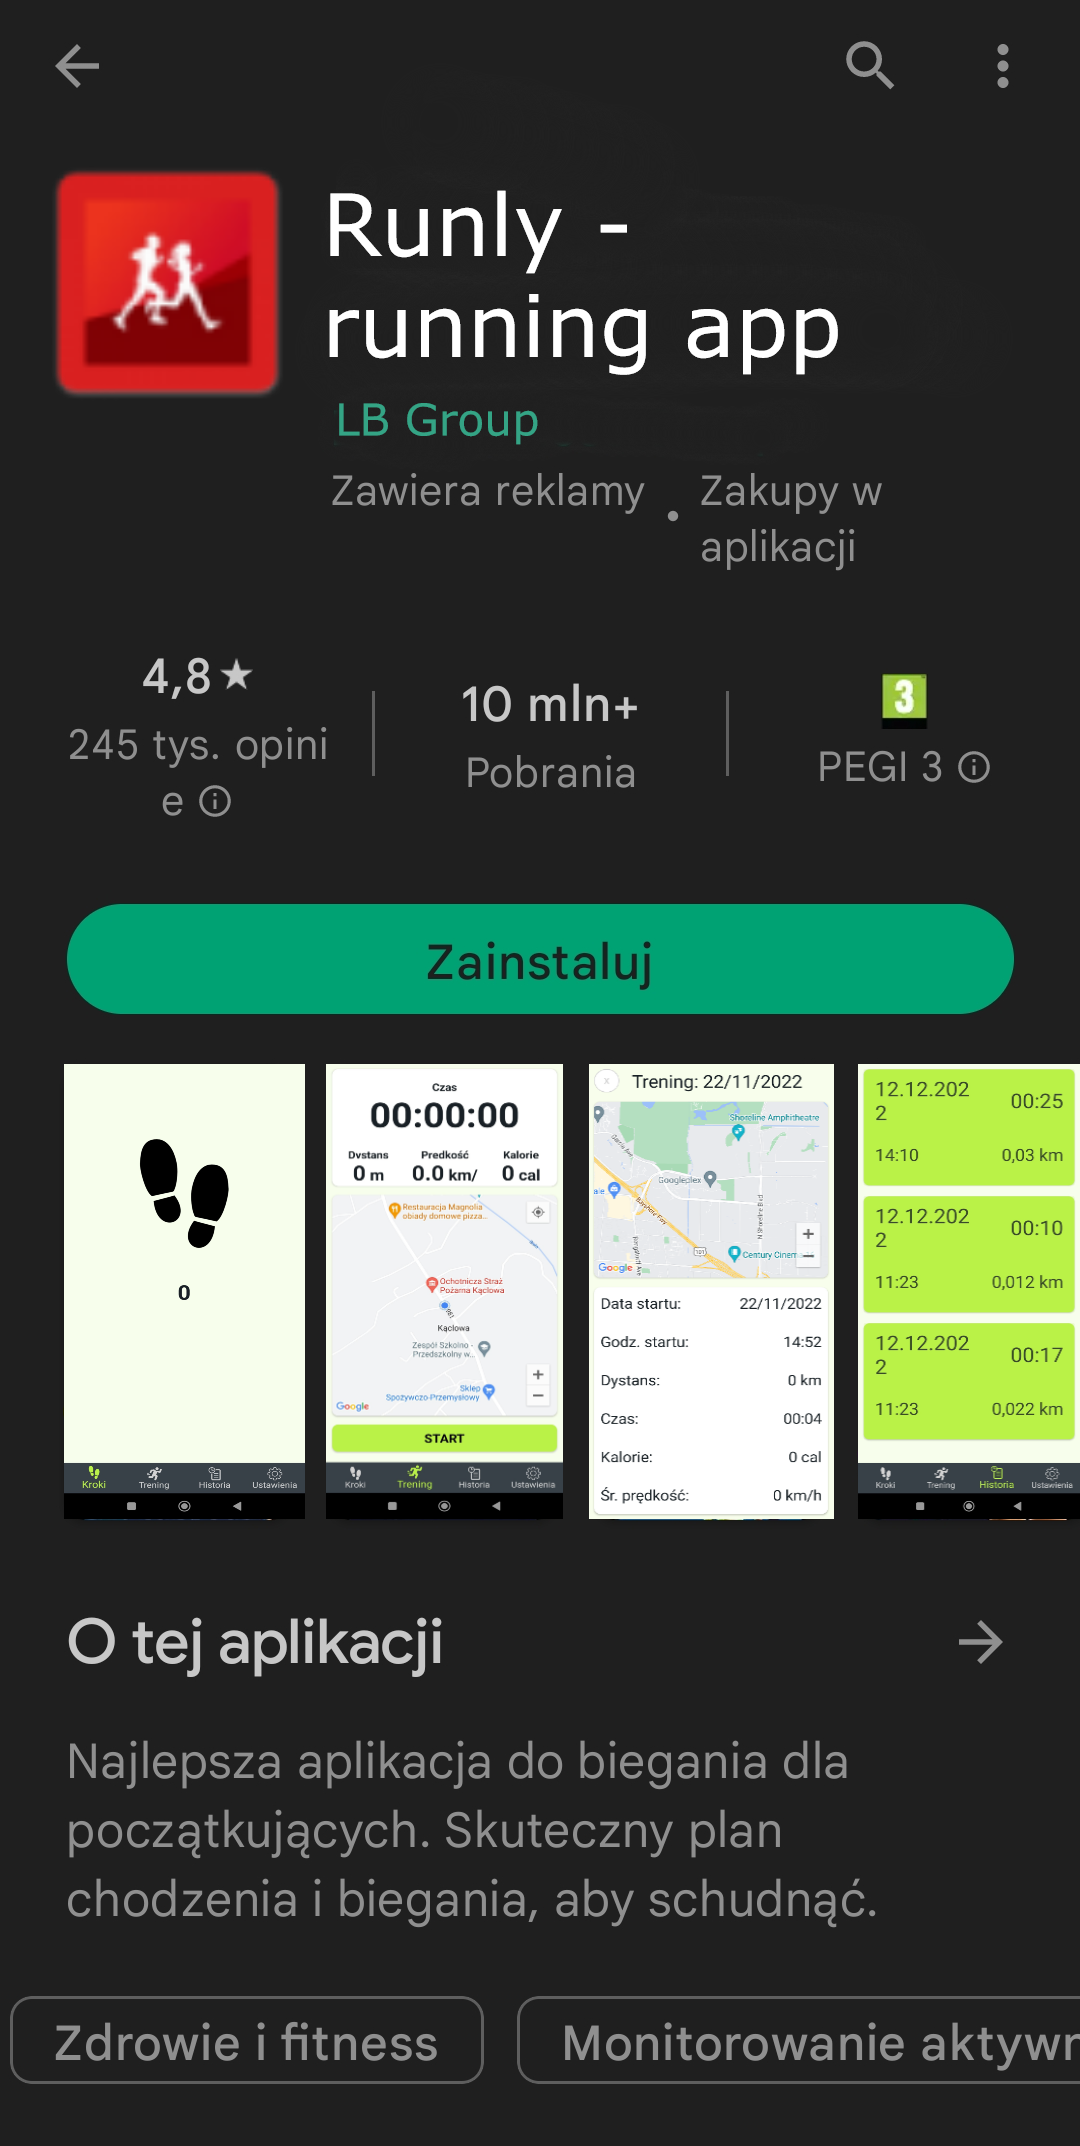
\includegraphics[width=.4\linewidth]{rys/runlyPS.png}
	\caption{Instalacja aplikacji ze sklepu Google Play}
	\label{rys:rysunek001epi}
\end{figure}

Przed uruchomieniem aplikacji, włącz w swoim telefonie moduł GPS (rys. \ref{rys:rysunek-r61}). Jest to niezbędne do poprawnego uruchomienia i działania aplikacji, gdyż korzysta ona z informacji o twojej aktualnej lokalizacji.
Uruchom aplikację Runly, klikając na jej ikonkę w menu aplikacji (rys. \ref{rys:rysunek-r62}).
Na ekranie pojawi się okienko Tracking Steps (rys. \ref{rys:rysunek-r63}), powiadamiające Cię o tym, że aplikacja rozpoczęła właśnie liczenie kroków jakie wykonujesz od momentu włączenia aplikacji do jej wyłączenia. Liczba kroków jest wyświetlana w zakładce Kroki (rys. \ref{rys:rysunek-r64}). W celu zalogowania do swojego konta użytkownika, wejdź w zakładkę Ustawienia (rys. \ref{rys:rysunek-r65}) i w odpowiednie pola wpisz swój login i hasło (rys. \ref{rys:rysunek-r66}). Wprowadz również swoją wagę (rys. \ref{rys:rysunek-r67}) (wymagany przedział to 10-150 kg) i wiek, gdyż na ich podstawie aplikacja obliczała będzie odpowiednie parametry twojego treningu. Gdy już to zrobiłeś, jesteś gotowy do treningu.
W celu rozpoczęcia treningu wejdź w zakładkę Trening i kliknij przycisk Start (rys. \ref{rys:rysunek-r68}). \\

\begin{figure}[!htb]
	\centering
	\begin{minipage}{.5\textwidth}
		\centering
		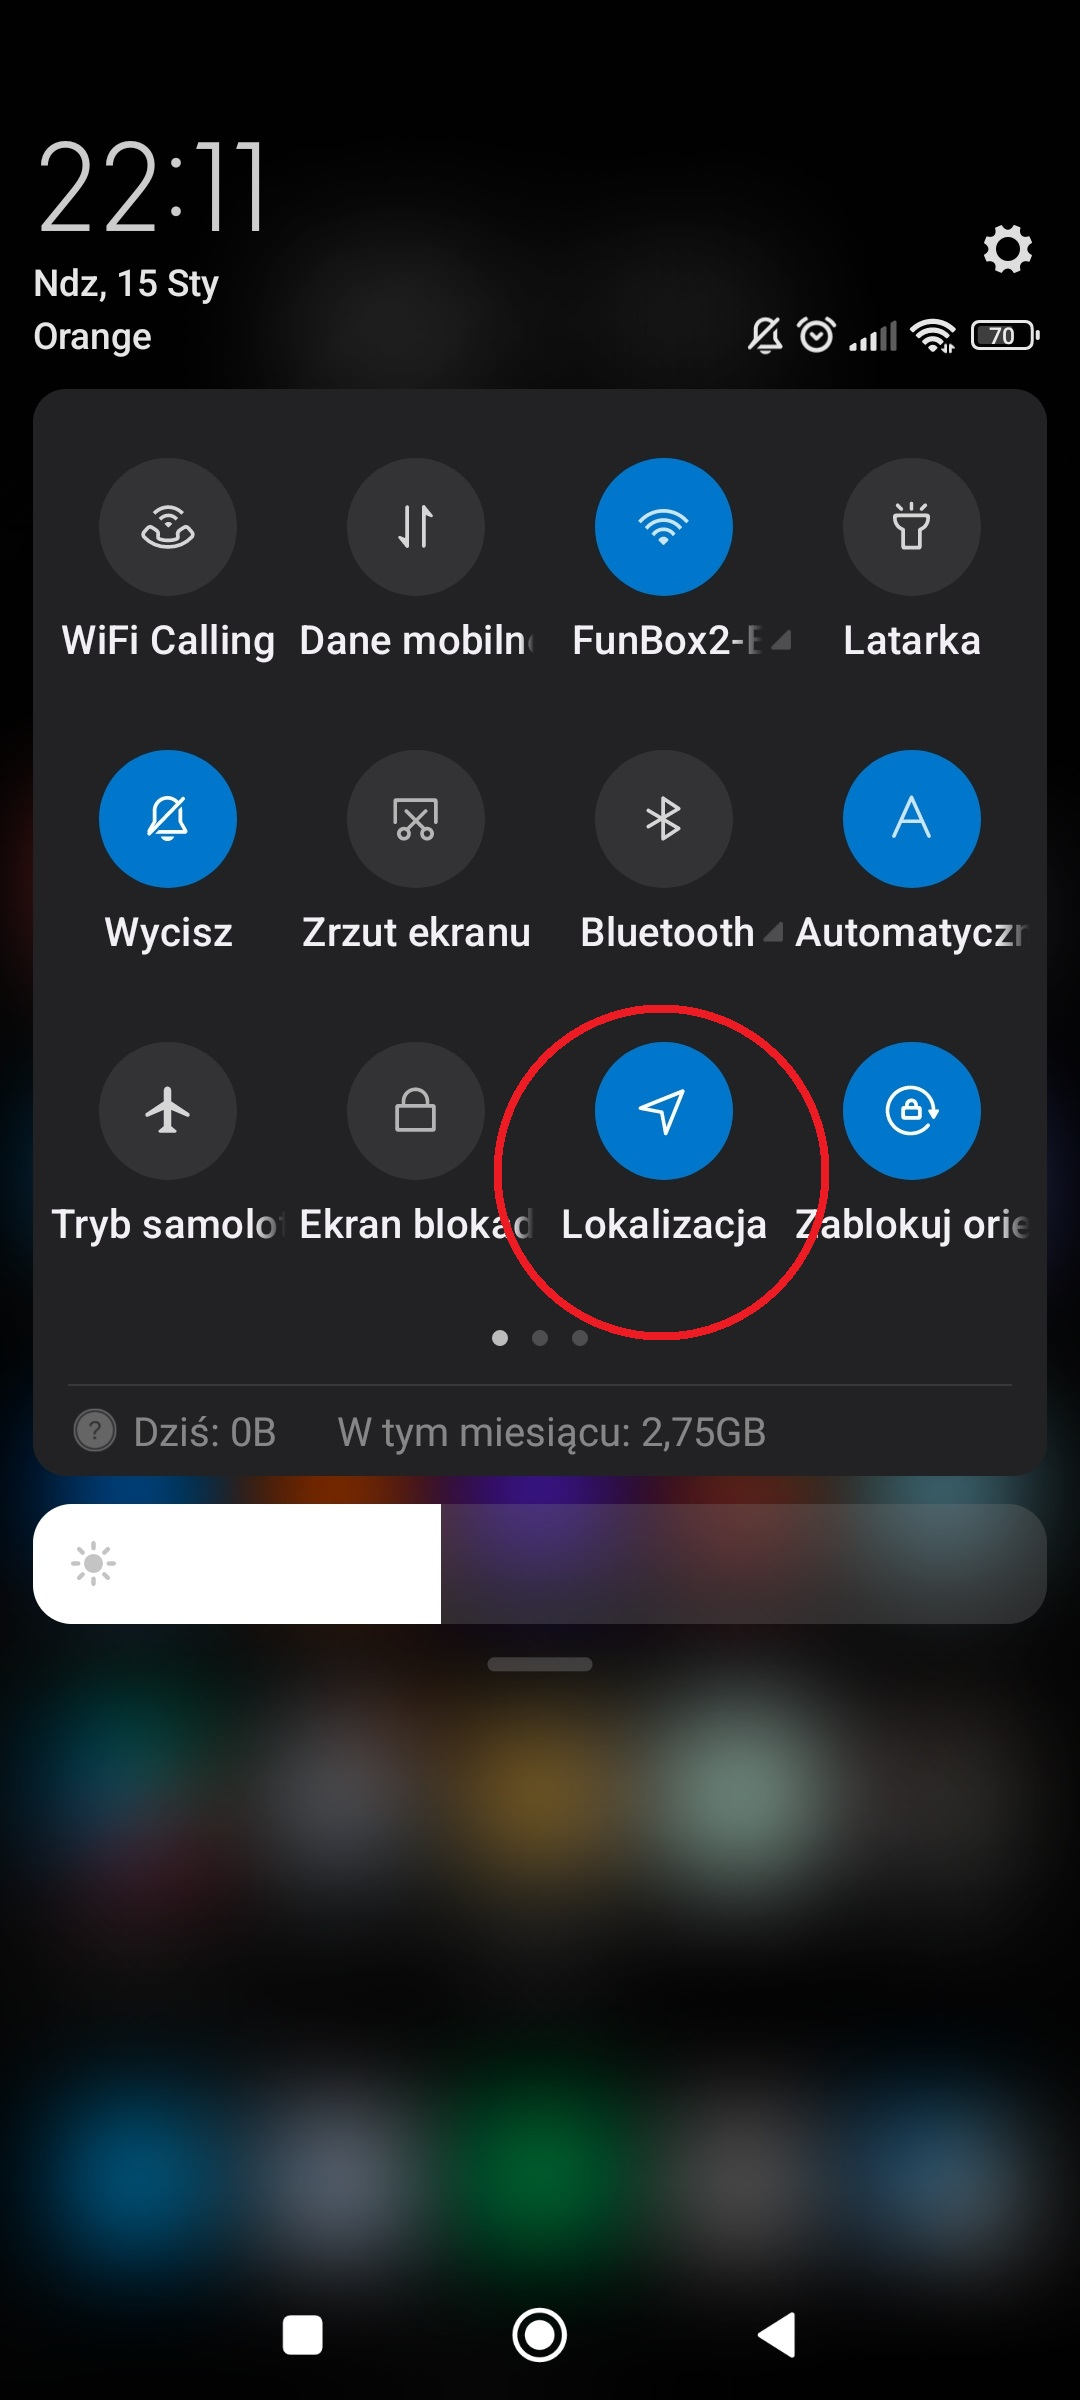
\includegraphics[width=.4\linewidth]{rys/r61.jpg}
		\caption{Włączenie GPS}
		\label{rys:rysunek-r61}
	\end{minipage}%
	\begin{minipage}{.5\textwidth}
		\centering
		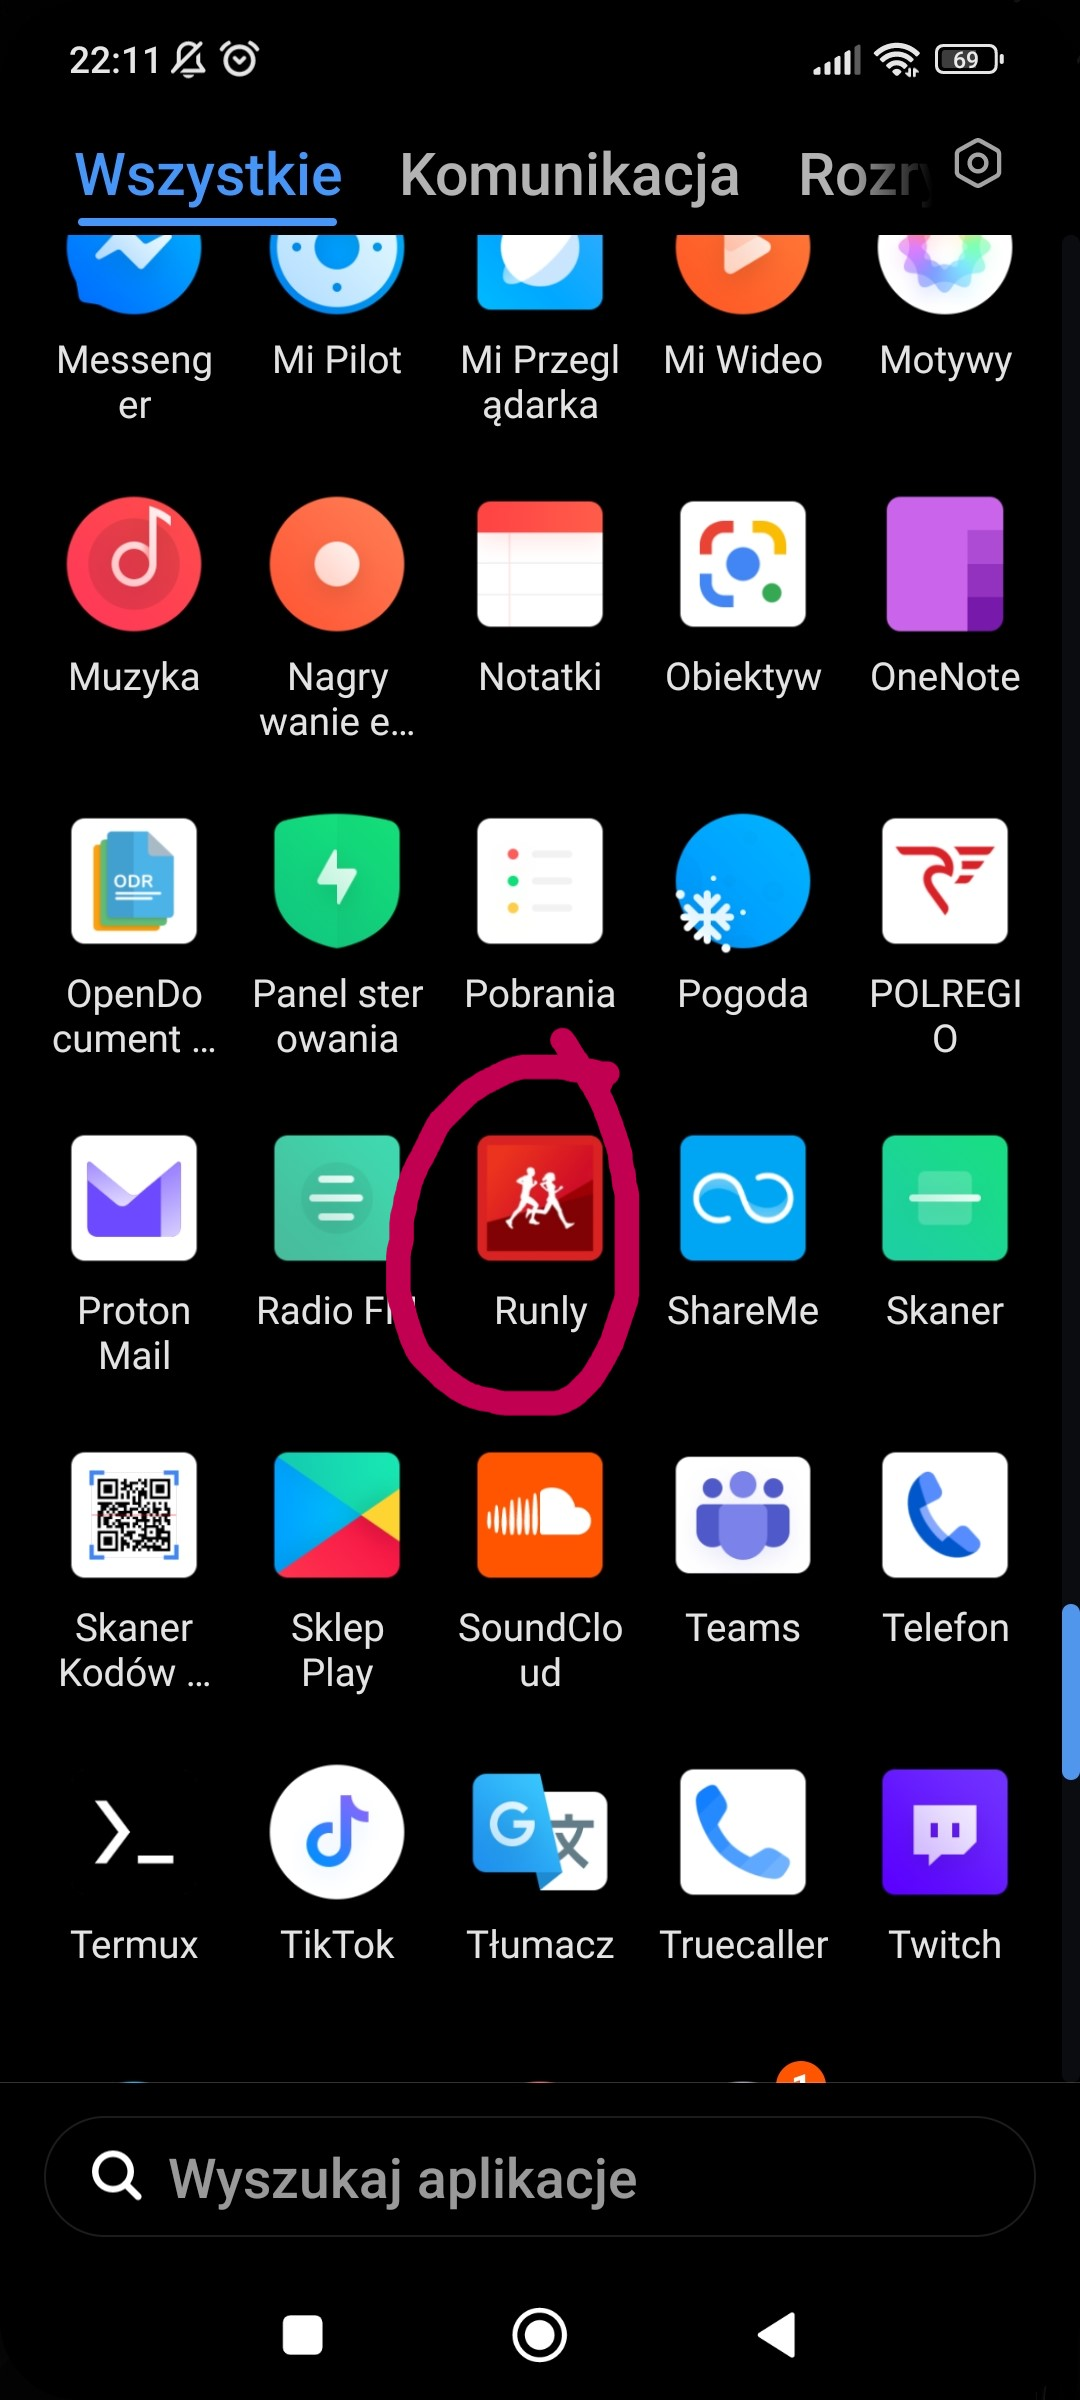
\includegraphics[width=.4\linewidth]{rys/r62.jpg}
		\caption{Uruchomienie aplikacji}
		\label{rys:rysunek-r62}
	\end{minipage}
\end{figure}

\begin{figure}[!htb]
	\centering
	\begin{minipage}{.5\textwidth}
		\centering
		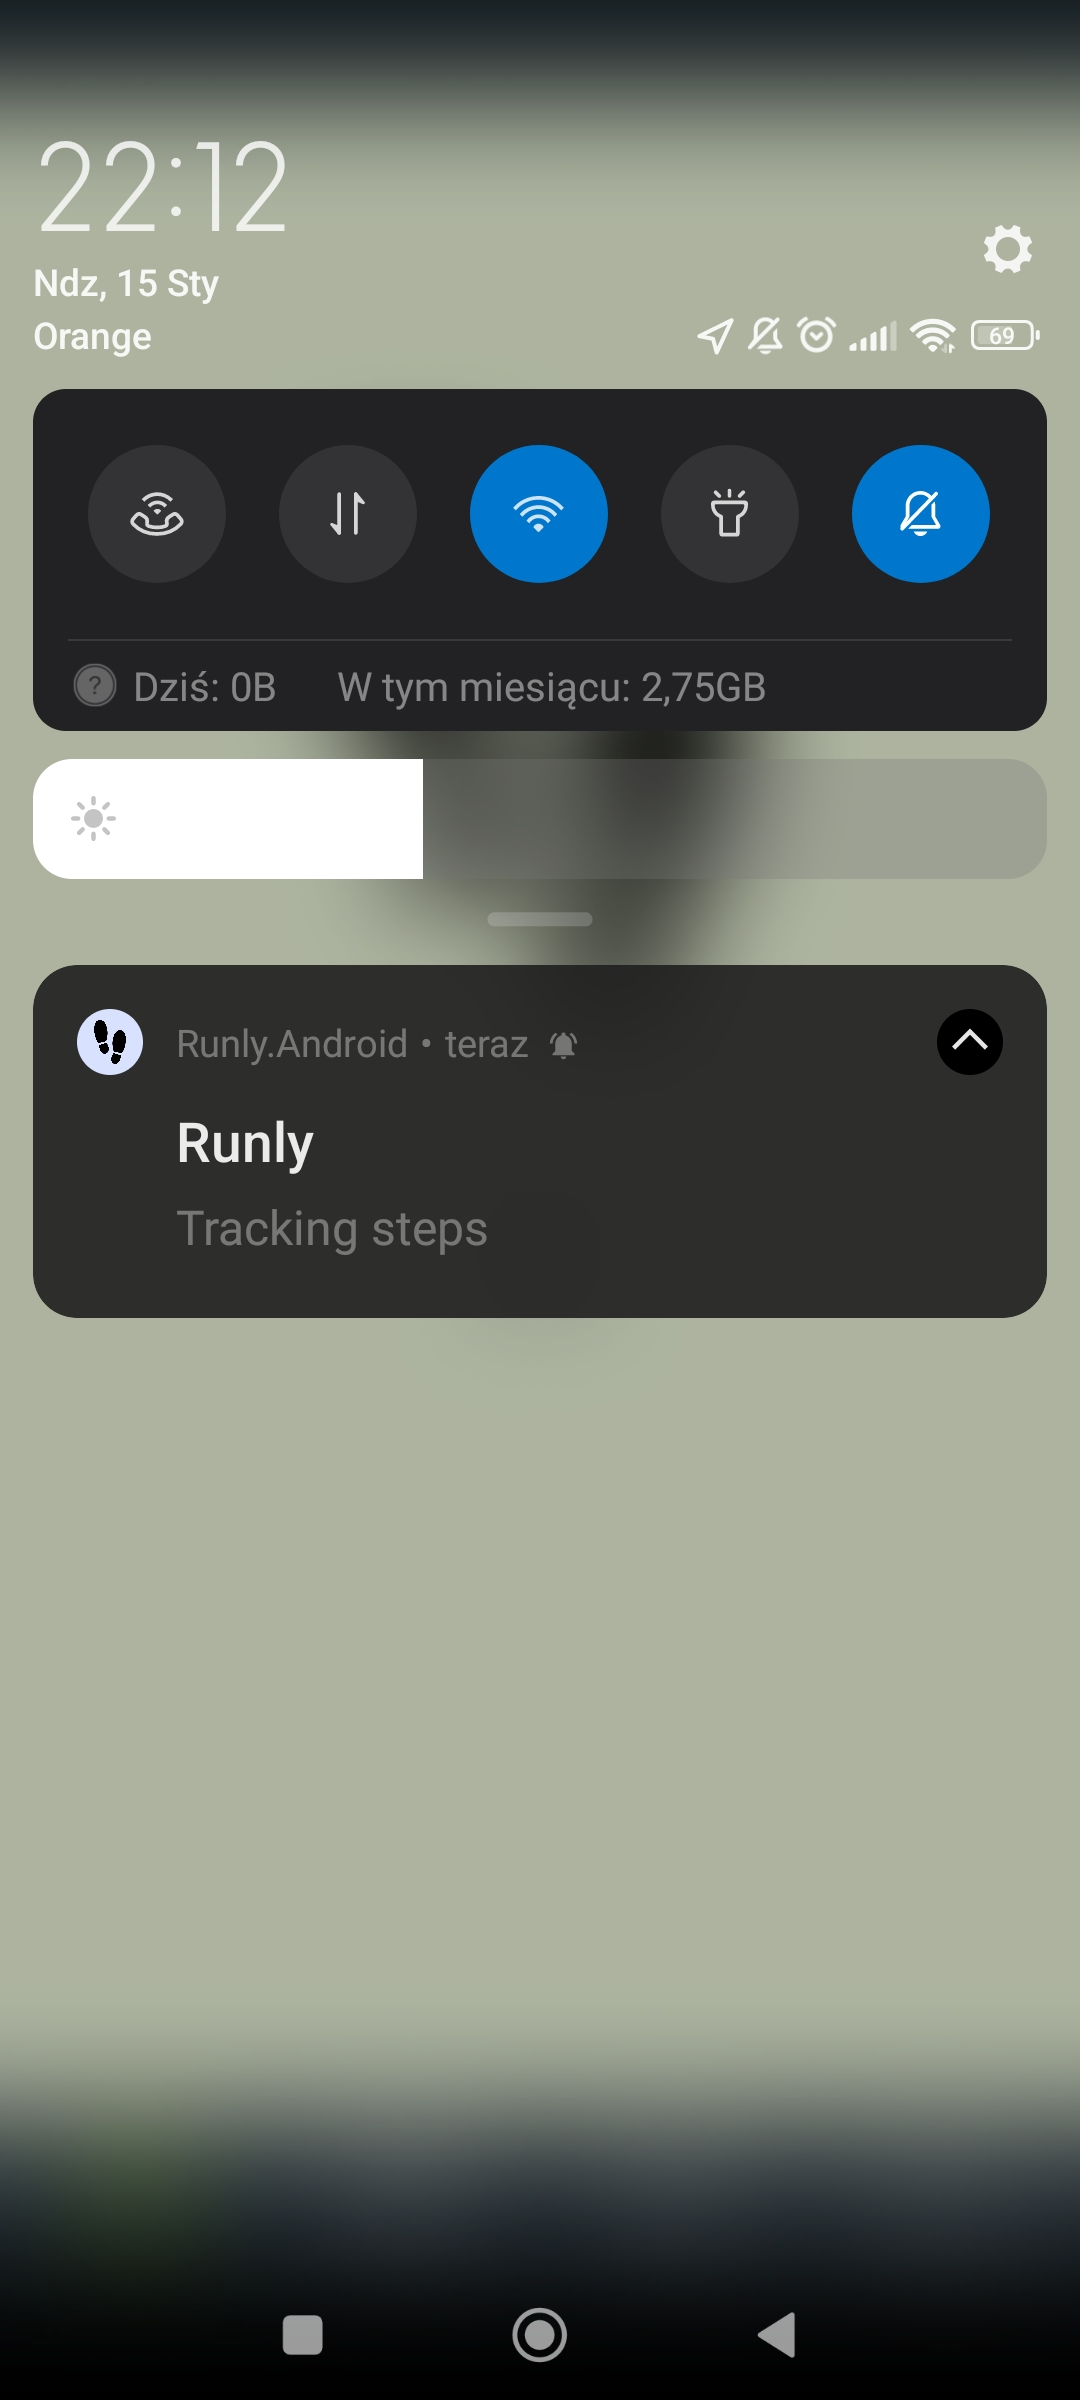
\includegraphics[width=.4\linewidth]{rys/r63.jpg}
		\caption{Powiadomienie Tracking Steps}
		\label{rys:rysunek-r63}
	\end{minipage}%
	\begin{minipage}{.5\textwidth}
		\centering
		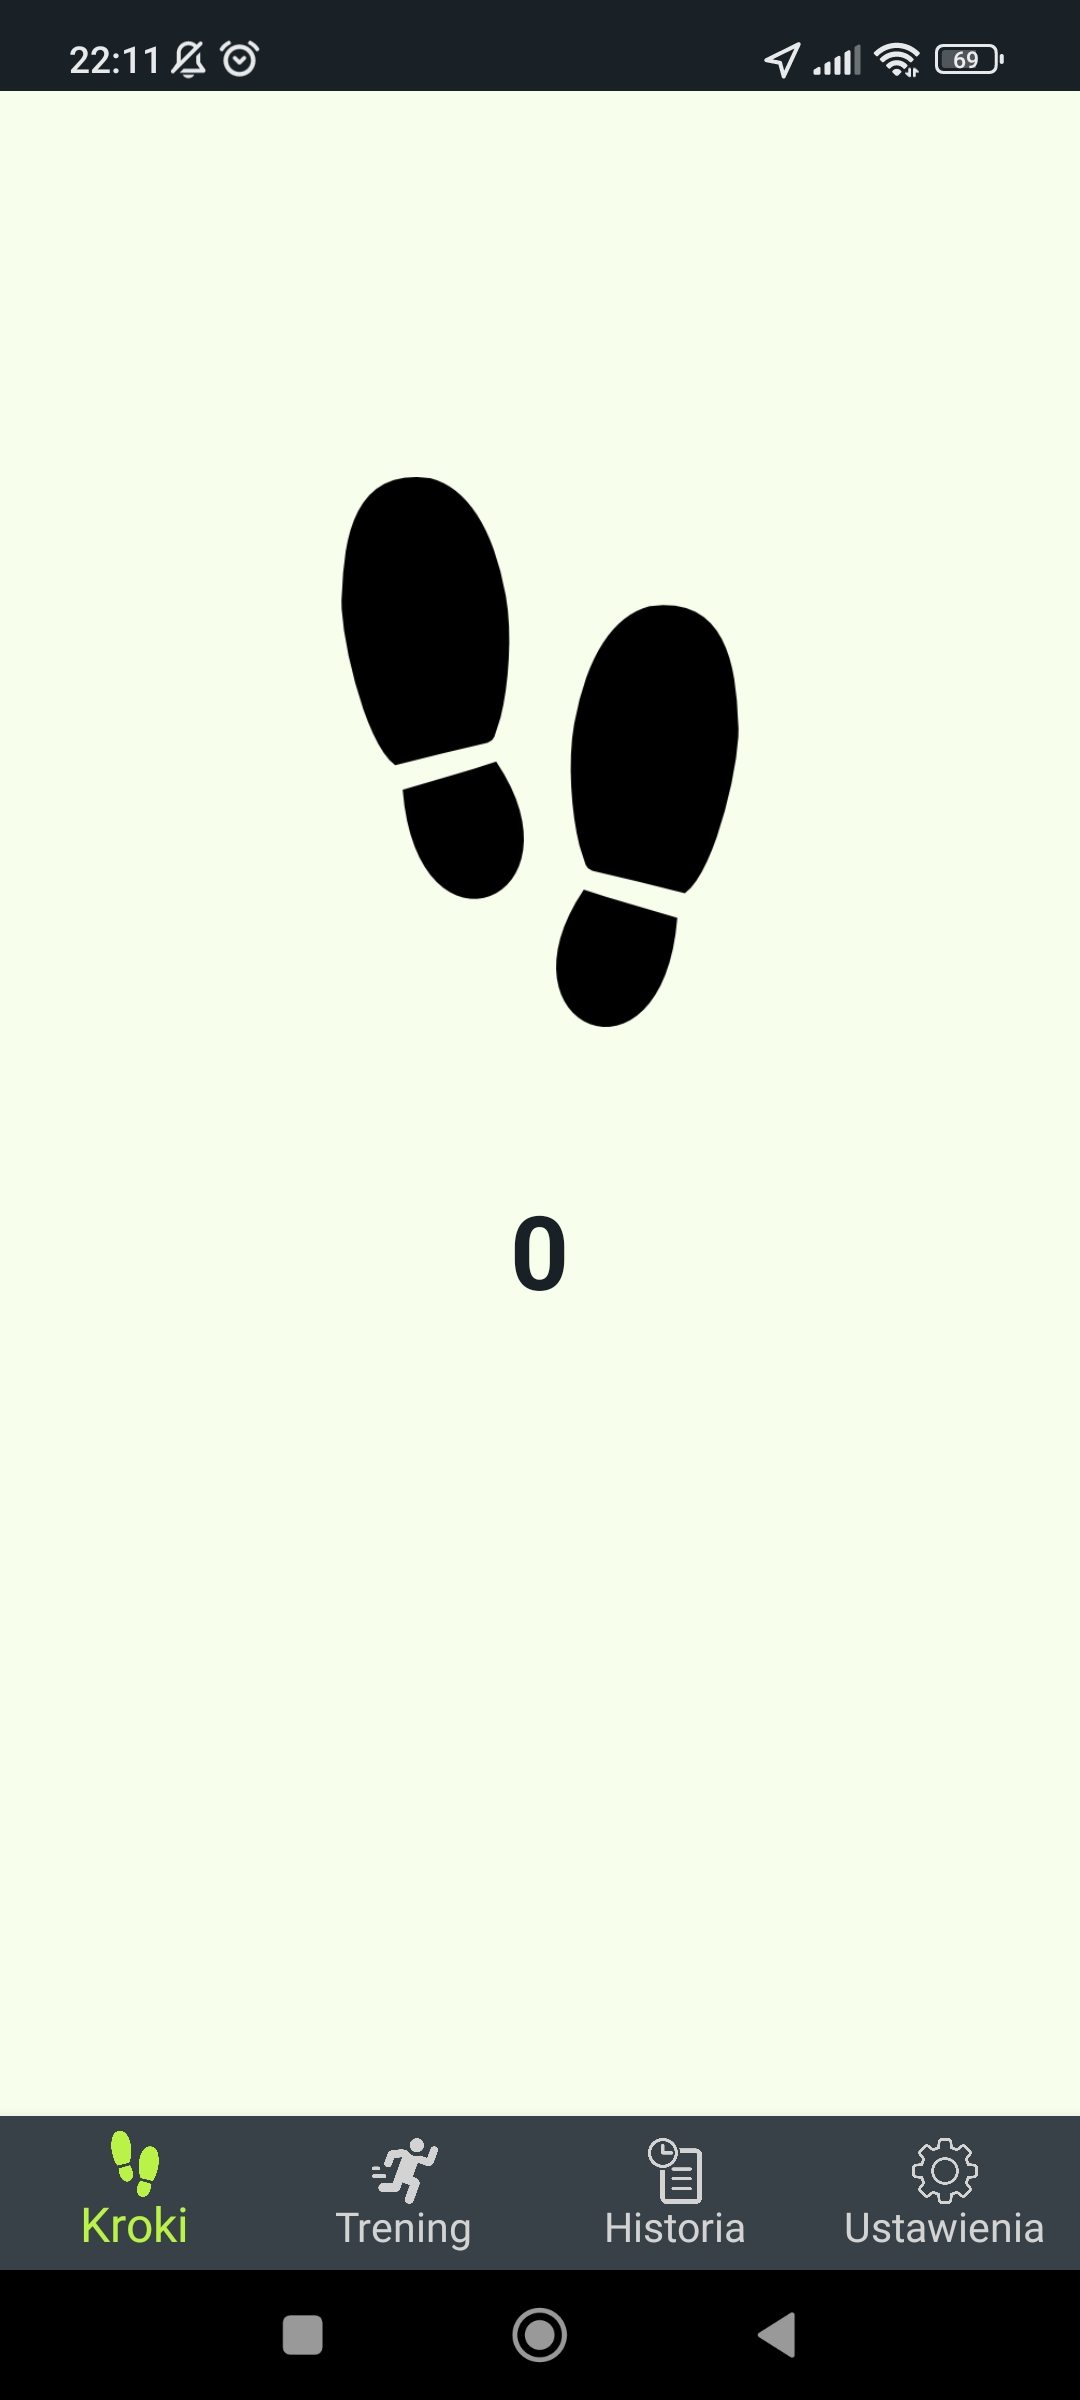
\includegraphics[width=.4\linewidth]{rys/r64.jpg}
		\caption{Wyświetlane kroki}
		\label{rys:rysunek-r64}
	\end{minipage}
\end{figure}

Rozpoczęcie treningu sprawia, że aplikacja zaczyna śledzić Twoje postępy w czasie rzeczywistym.
Na ekranie rozpoczyna  się odliczanie i wyświetlanie parametrów treningu, takich jak czas, dystans, prędkość. W zakładce Kroki możesz sprawdzić ilość wykonanych kroków zarówno od włączenia aplikacji jak i od momentu rozpoczęcia treningu (rys. \ref{rys:rysunek-r610}). 

\begin{figure}[!htb]
	\centering
	\begin{minipage}{.5\textwidth}
		\centering
		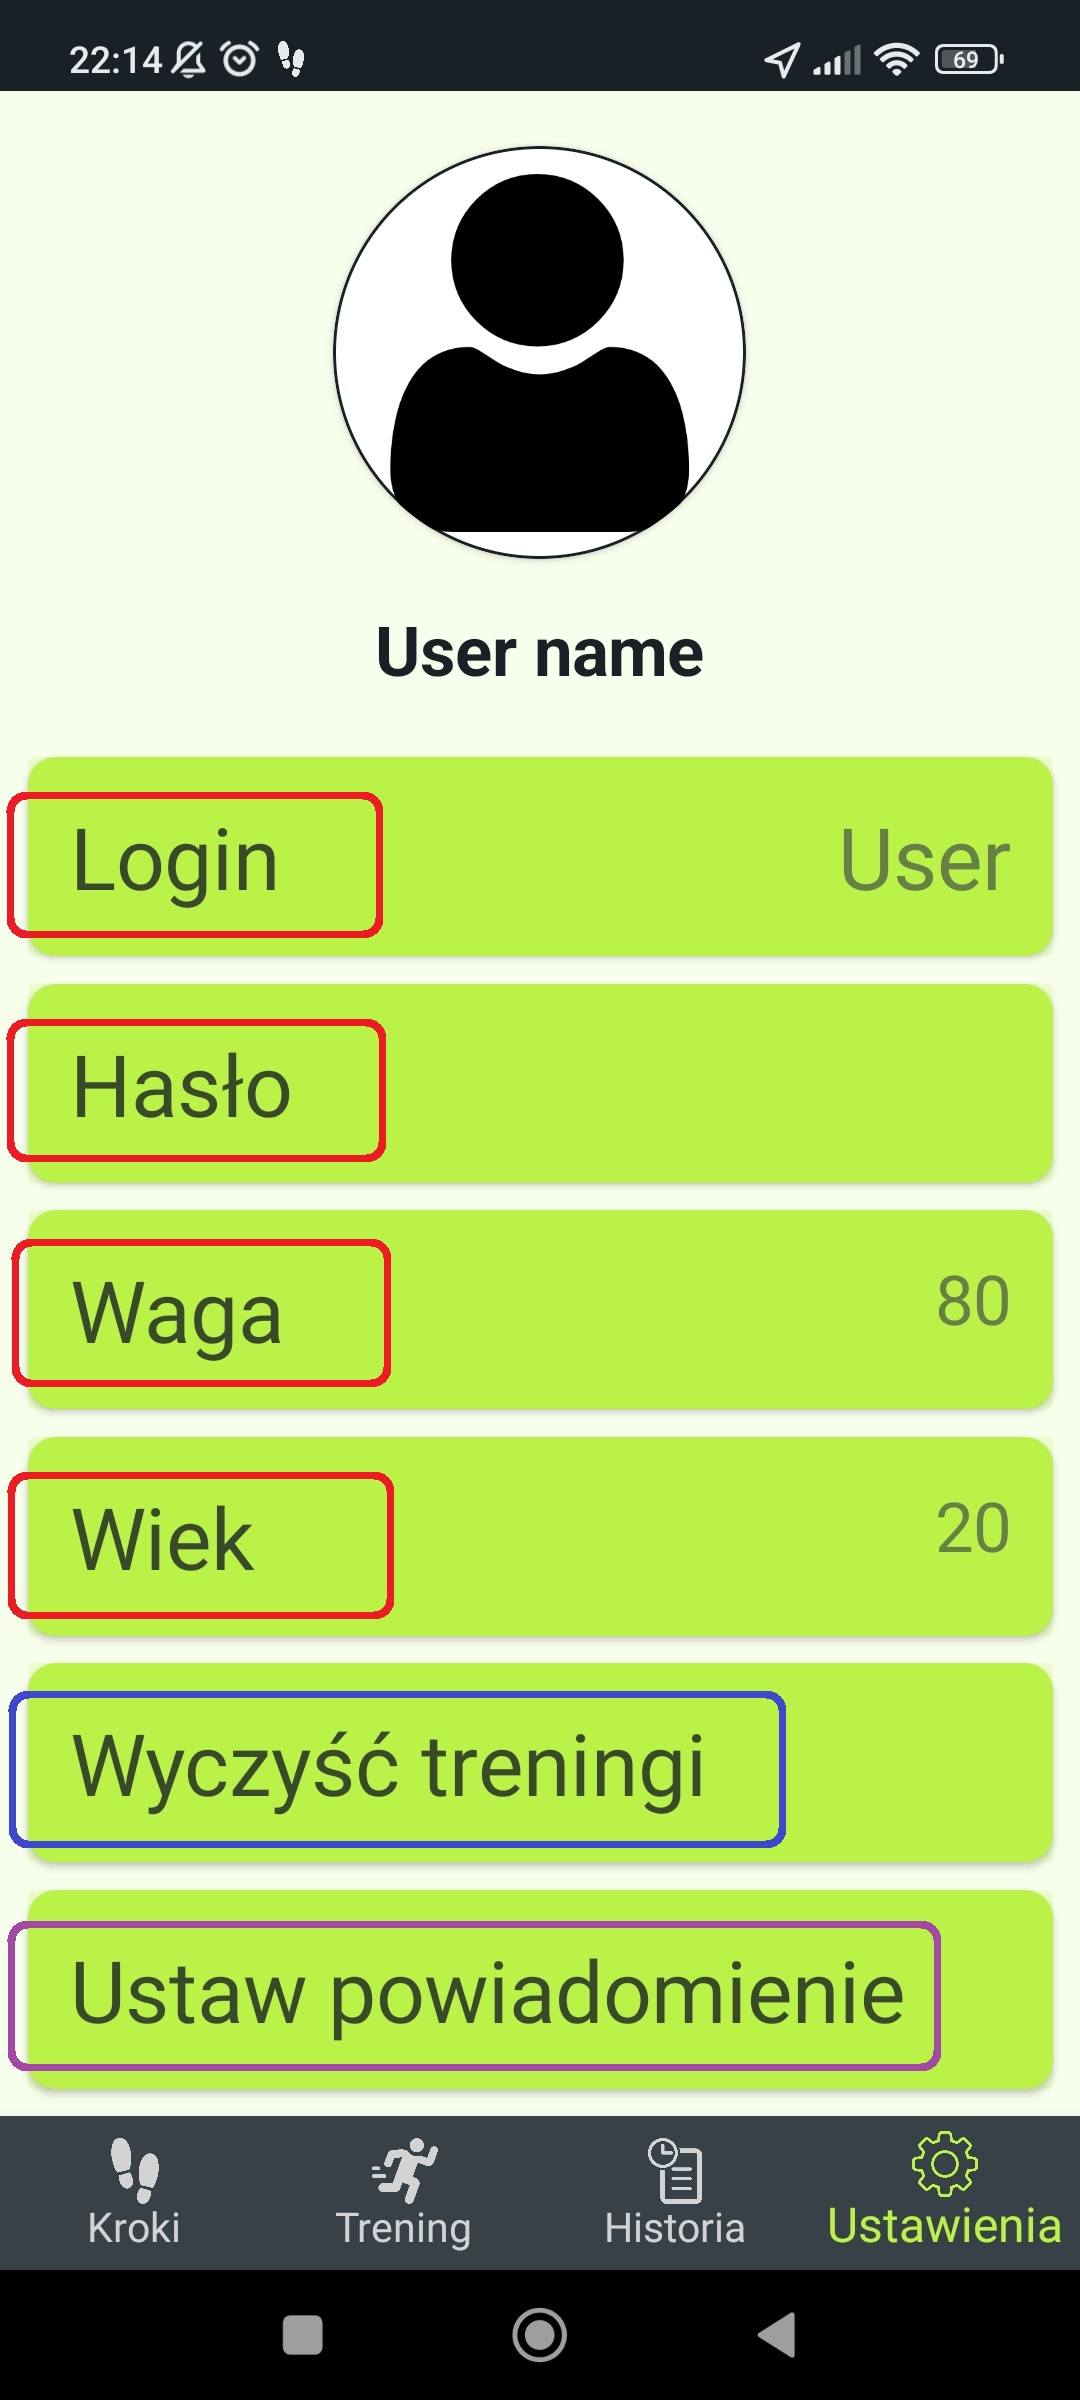
\includegraphics[width=.4\linewidth]{rys/r65.jpg}
		\caption{Zakładka Ustawienia}
		\label{rys:rysunek-r65}
	\end{minipage}%
	\begin{minipage}{.5\textwidth}
		\centering
		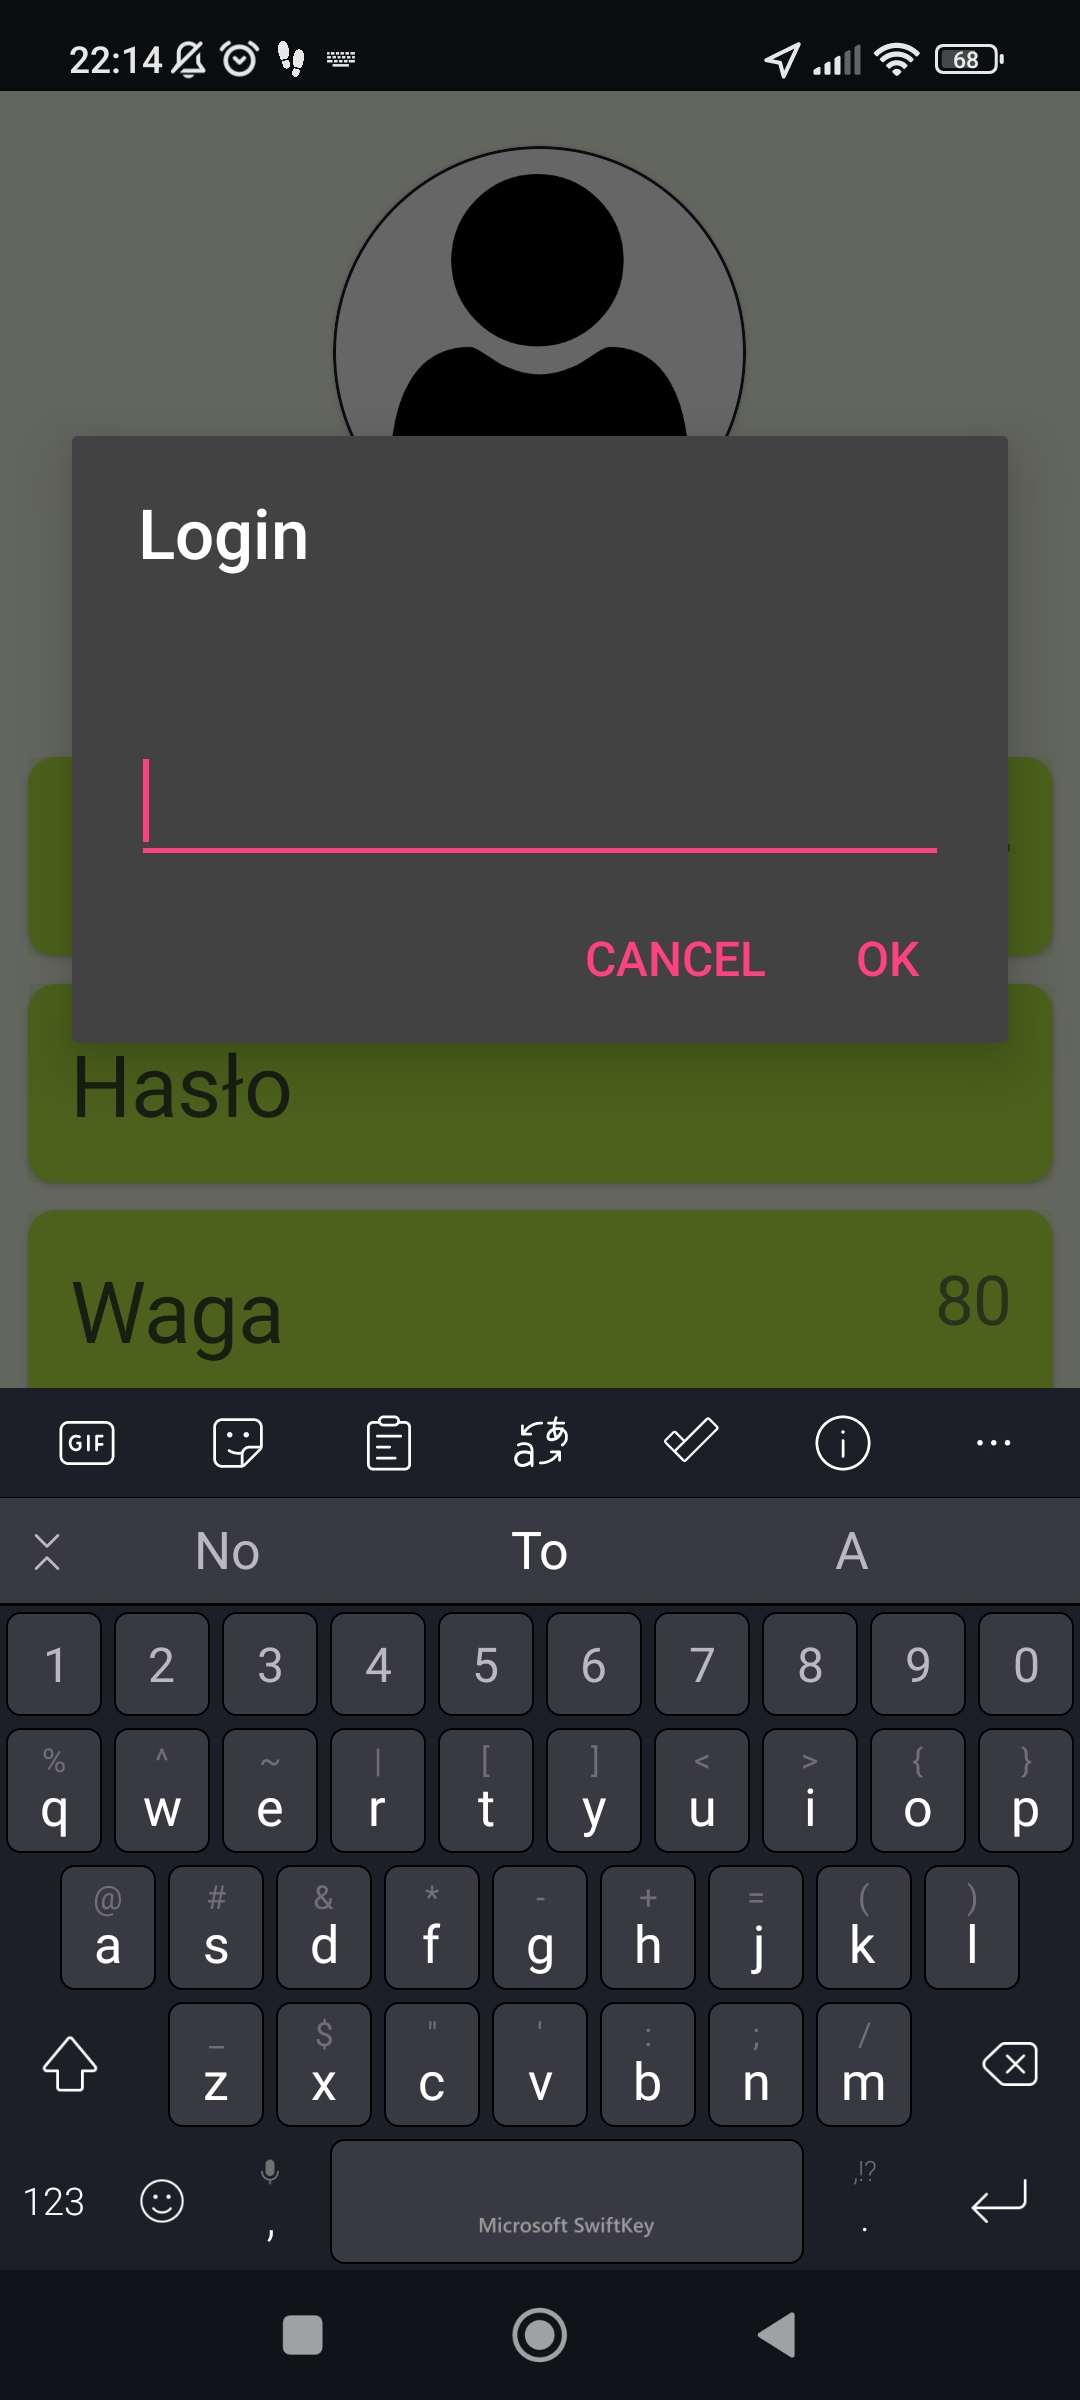
\includegraphics[width=.4\linewidth]{rys/r66.jpg}
		\caption{Wpisanie loginu}
		\label{rys:rysunek-r66}
	\end{minipage}
\end{figure}

\begin{figure}[!htb]
	\centering
	\begin{minipage}{.5\textwidth}
		\centering
		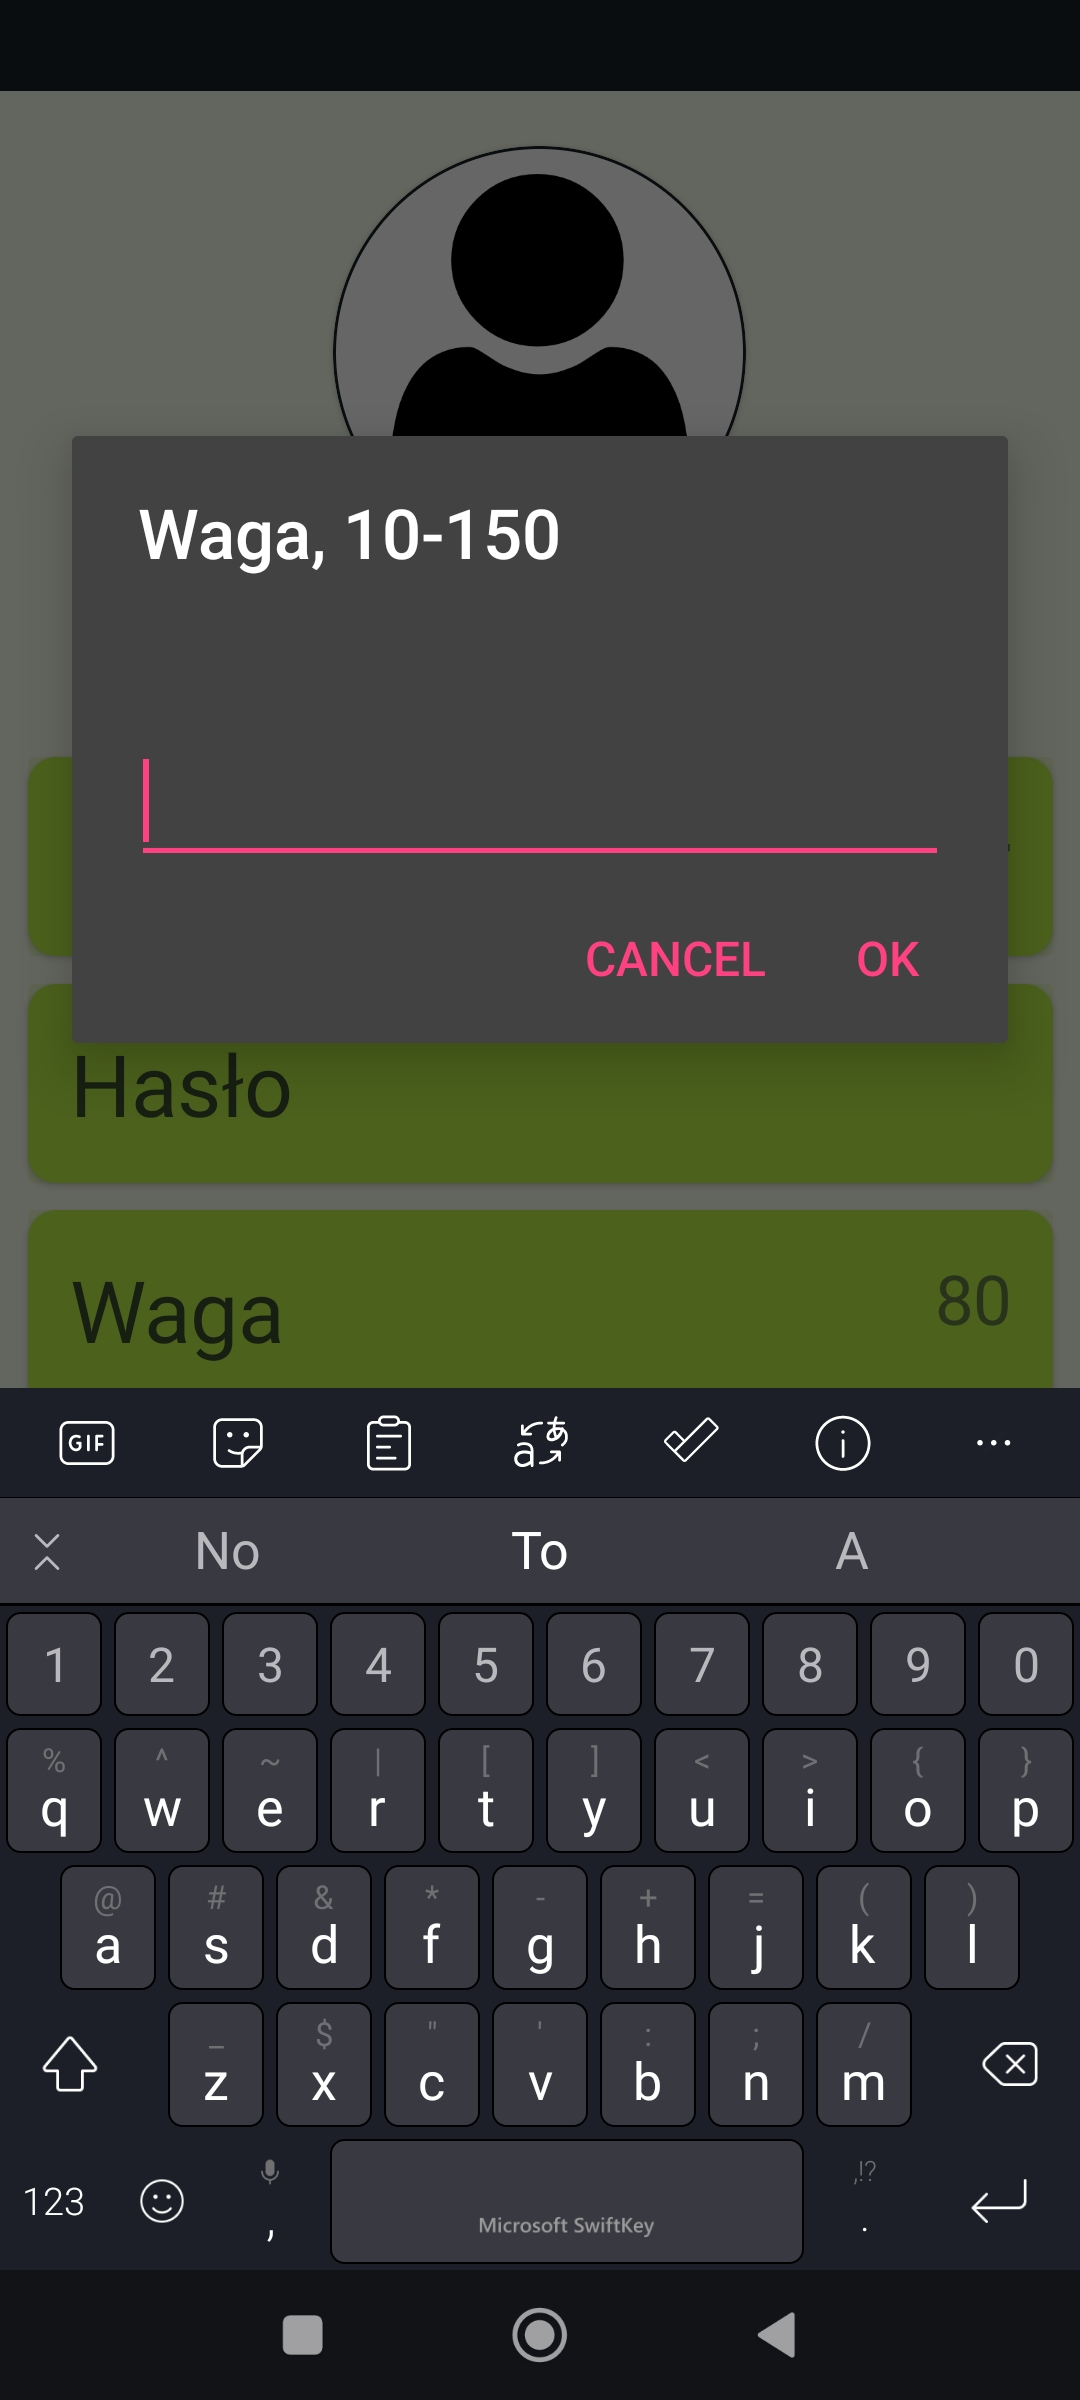
\includegraphics[width=.4\linewidth]{rys/r67.jpg}
		\caption{Wpisanie swojej wagi}
		\label{rys:rysunek-r67}
	\end{minipage}%
	\begin{minipage}{.5\textwidth}
		\centering
		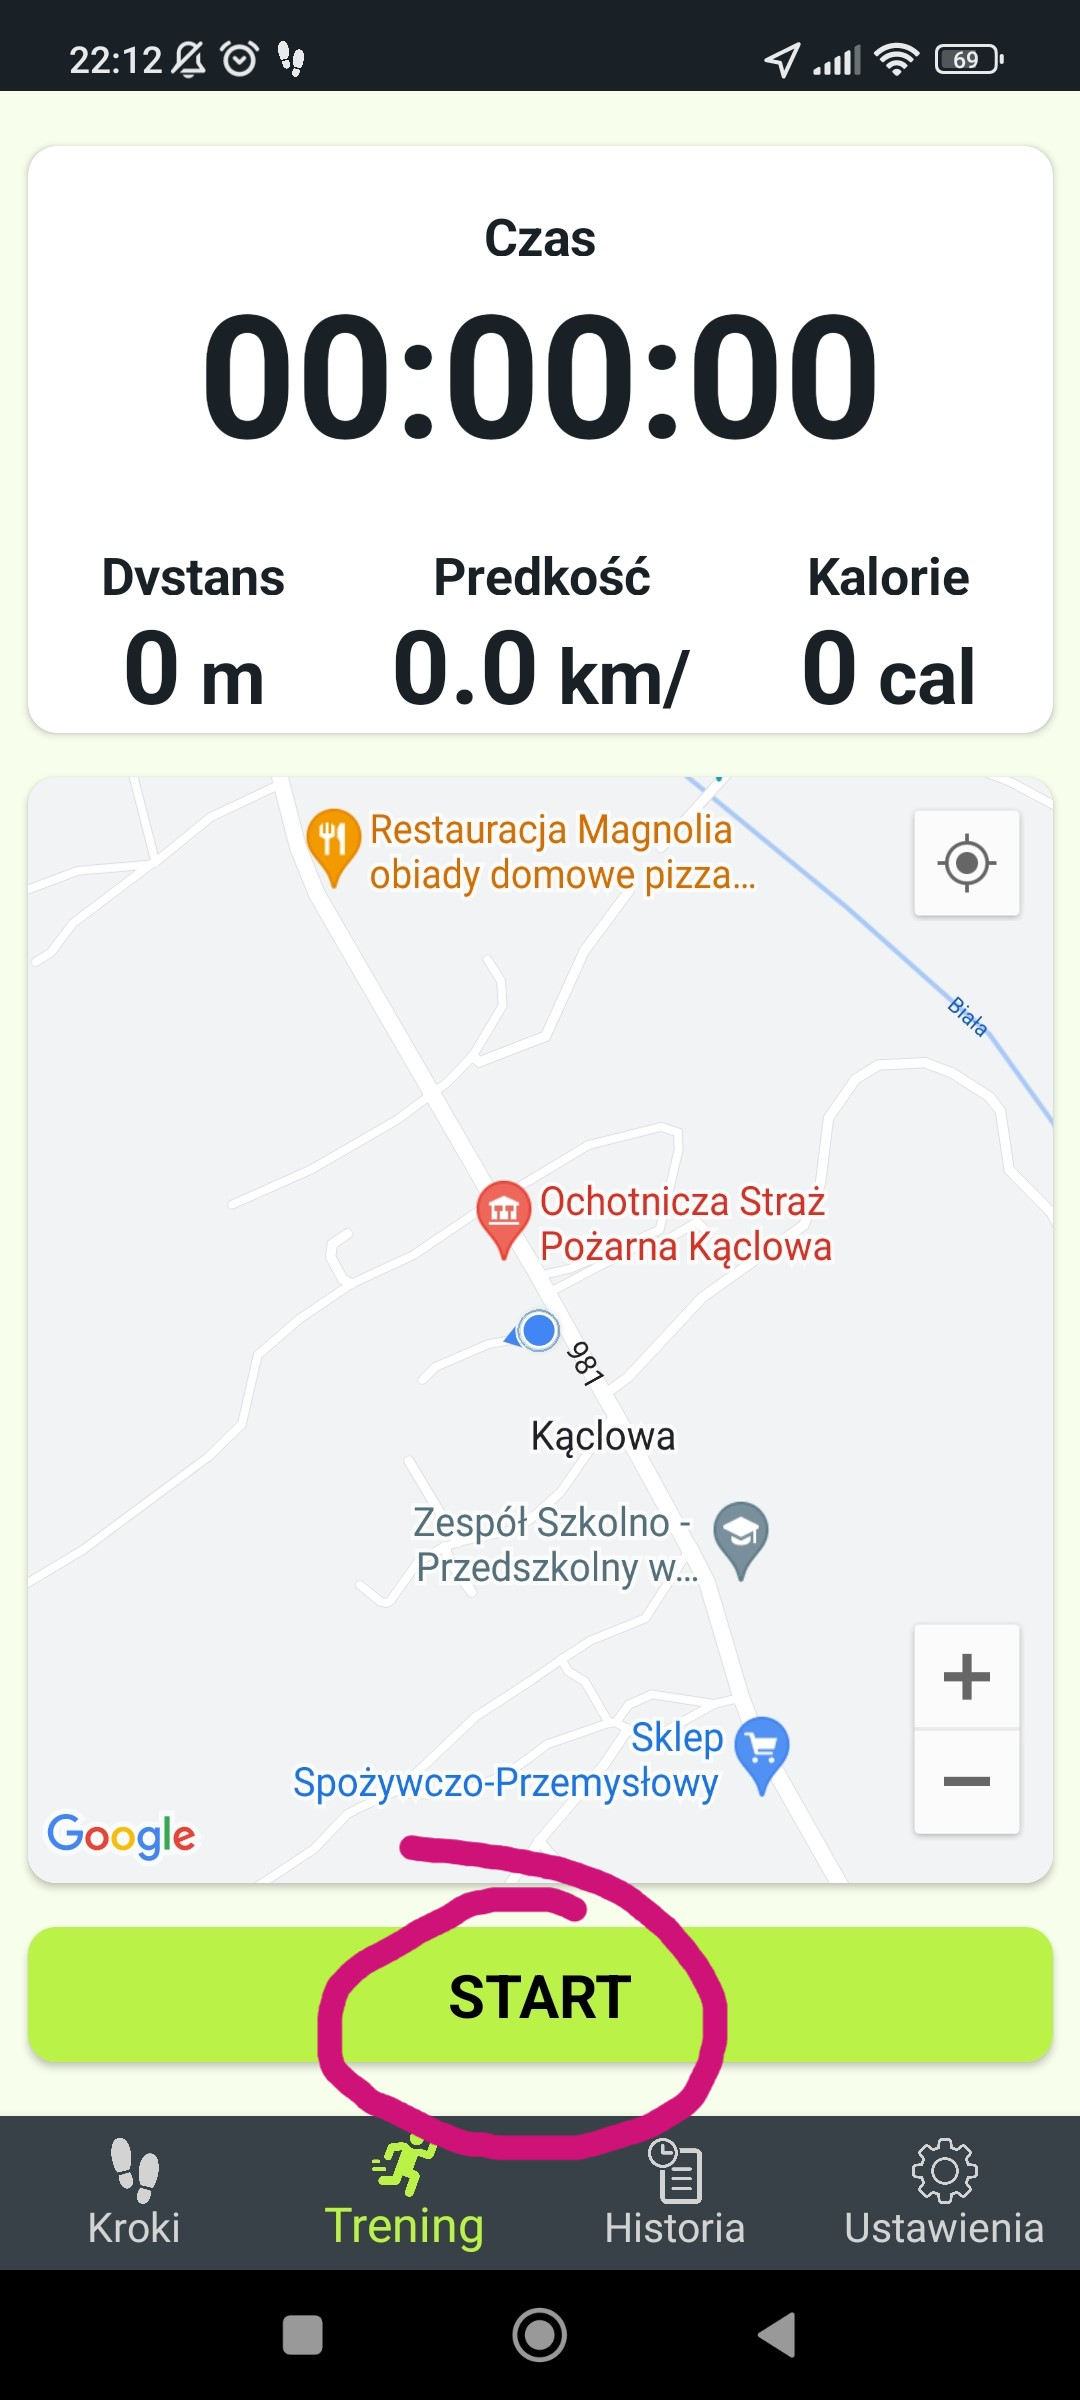
\includegraphics[width=.4\linewidth]{rys/r68.jpg}
		\caption{Rozpoczęcie treningu}
		\label{rys:rysunek-r68}
	\end{minipage}
\end{figure}

Jeśli nadejdzie taka potrzeba, w każdej chwili możesz zatrzymać trening przyciskiem Stop (rys. \ref{rys:rysunek-r69}). Wstrzyma to liczenie parametrów treningu. Od tego momentu masz dwie możliwości: wznowienie treningu przyciskiem Wznów lub zakończenie treningu przyciskiem Koniec (rys. \ref{rys:rysunek-r612}). Naciśnięcie tego pierwszego po prostu wznawia trening od momentu wstrzymania, kontynuując obliczanie parametrów.  Naciśnięcie drugiego kończy cały trening, a na ekranie wyświetlone zostaje okno z podsumowaniem treningu (rys. \ref{rys:rysunek-r613}).

\begin{figure}[!htb]
	\centering
	\begin{minipage}{.5\textwidth}
		\centering
		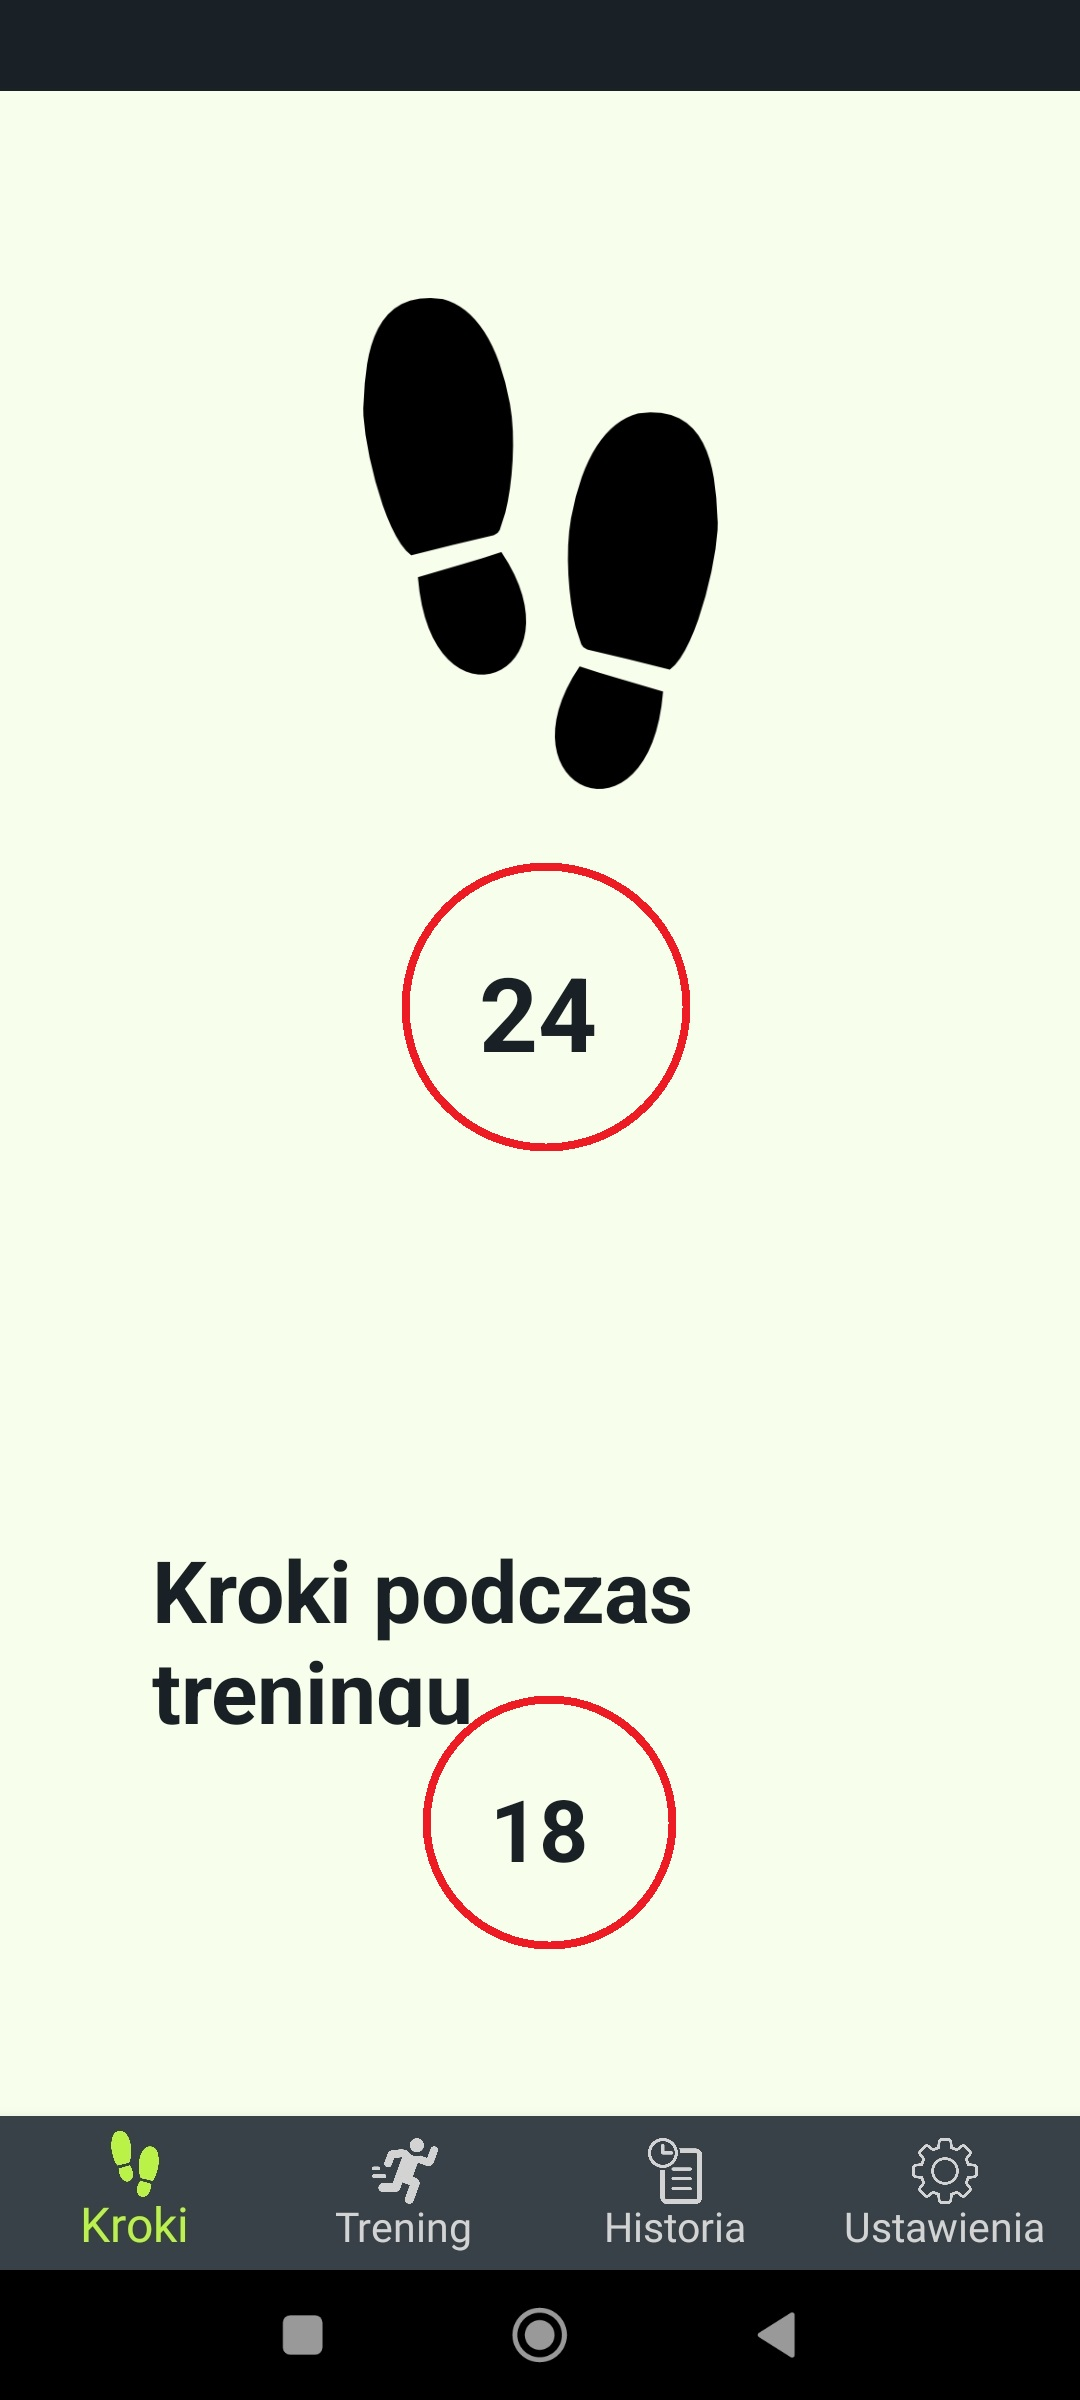
\includegraphics[width=.4\linewidth]{rys/r610.jpg}
		\caption{Kroki podczas treningu}
		\label{rys:rysunek-r610}
	\end{minipage}%
	\begin{minipage}{.5\textwidth}
		\centering
		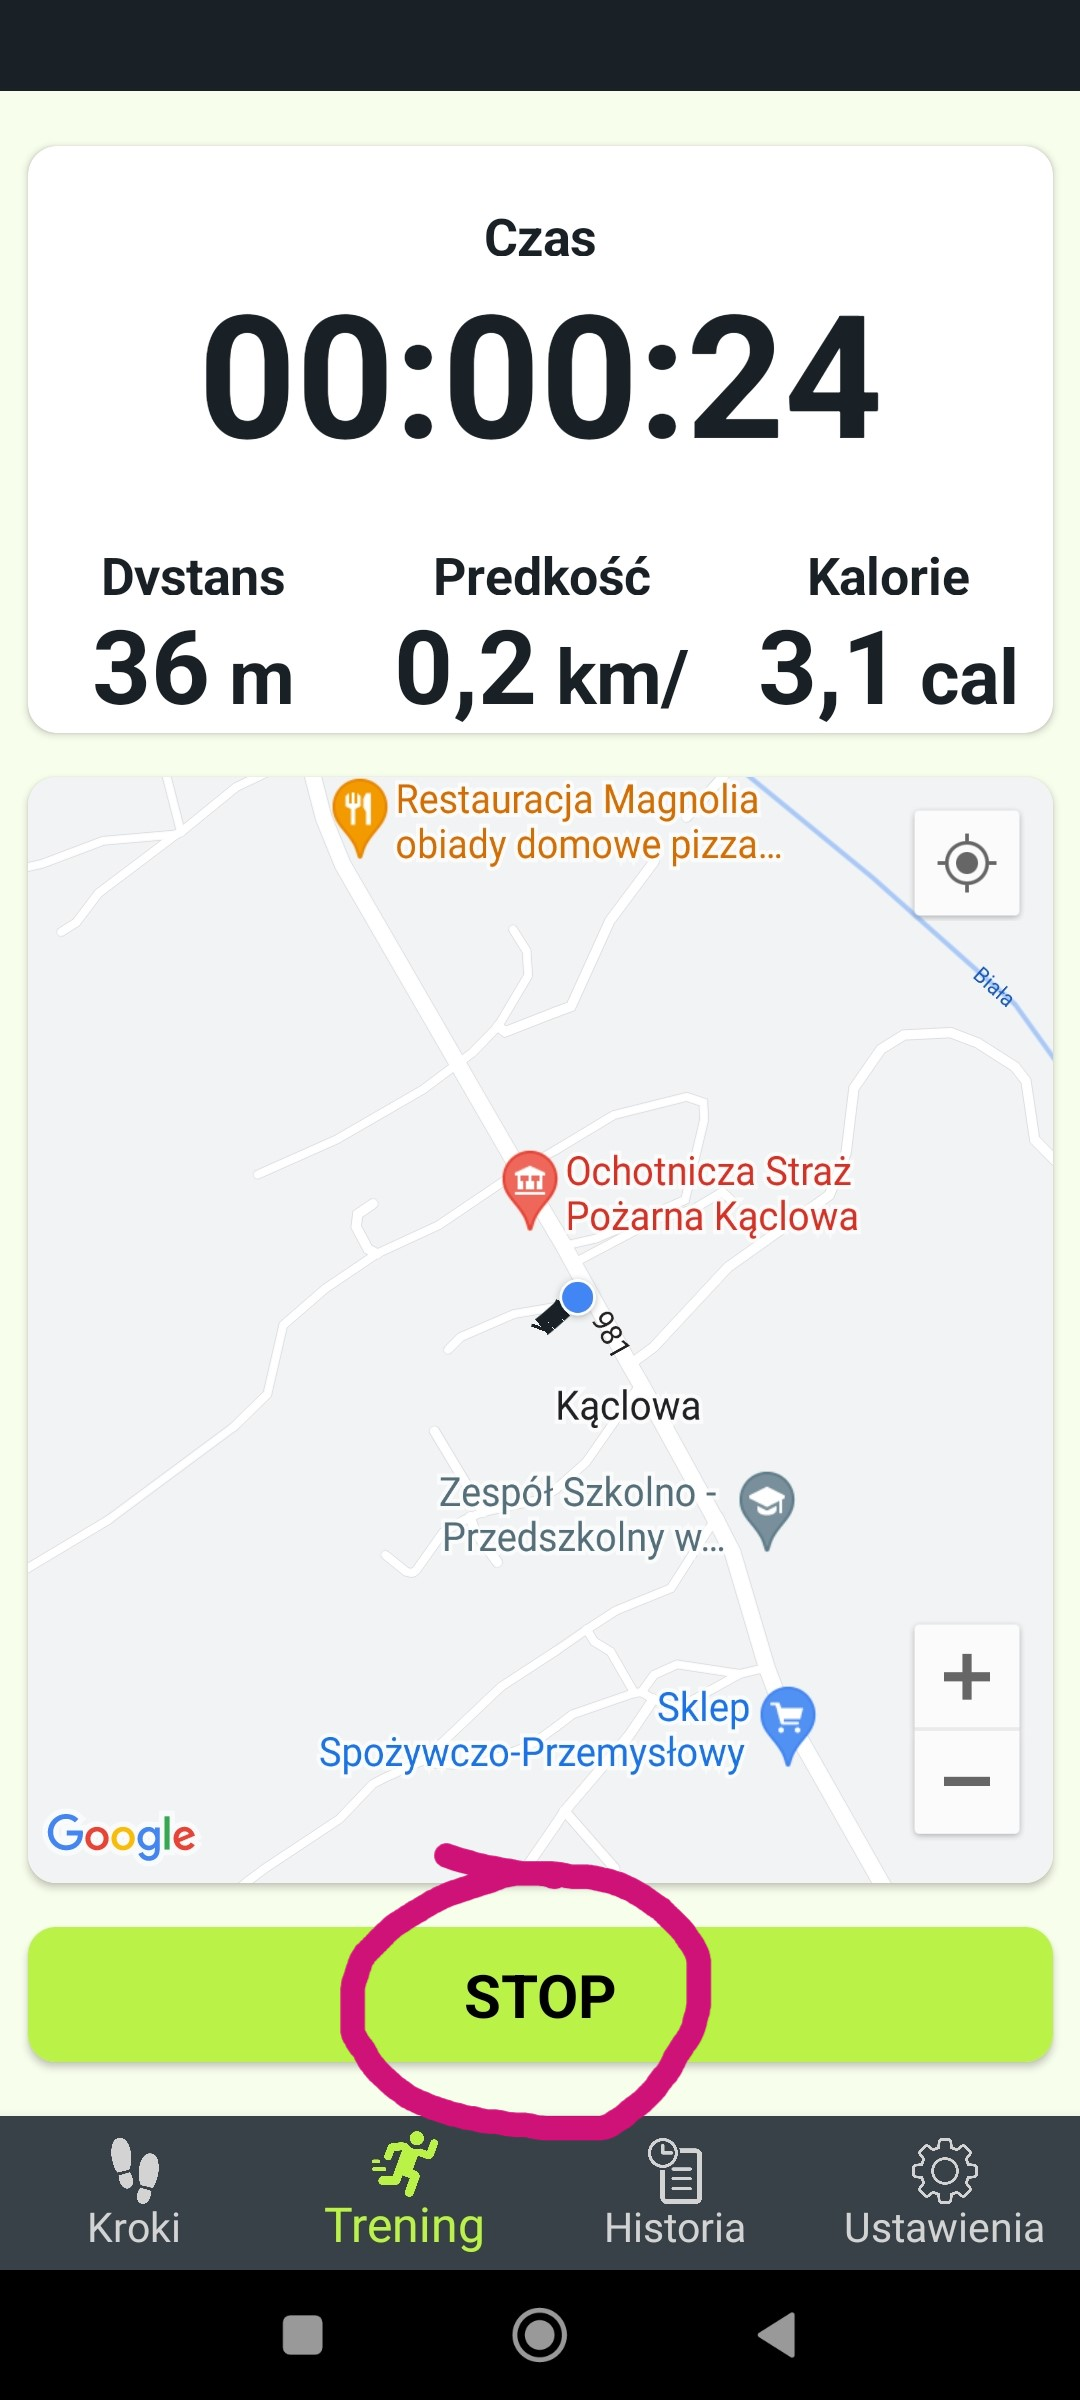
\includegraphics[width=.4\linewidth]{rys/r69.jpg}
		\caption{Wstrzymanie treningu}
		\label{rys:rysunek-r69}
	\end{minipage}
\end{figure}

\begin{figure}[!htb]
	\centering
	\begin{minipage}{.5\textwidth}
		\centering
		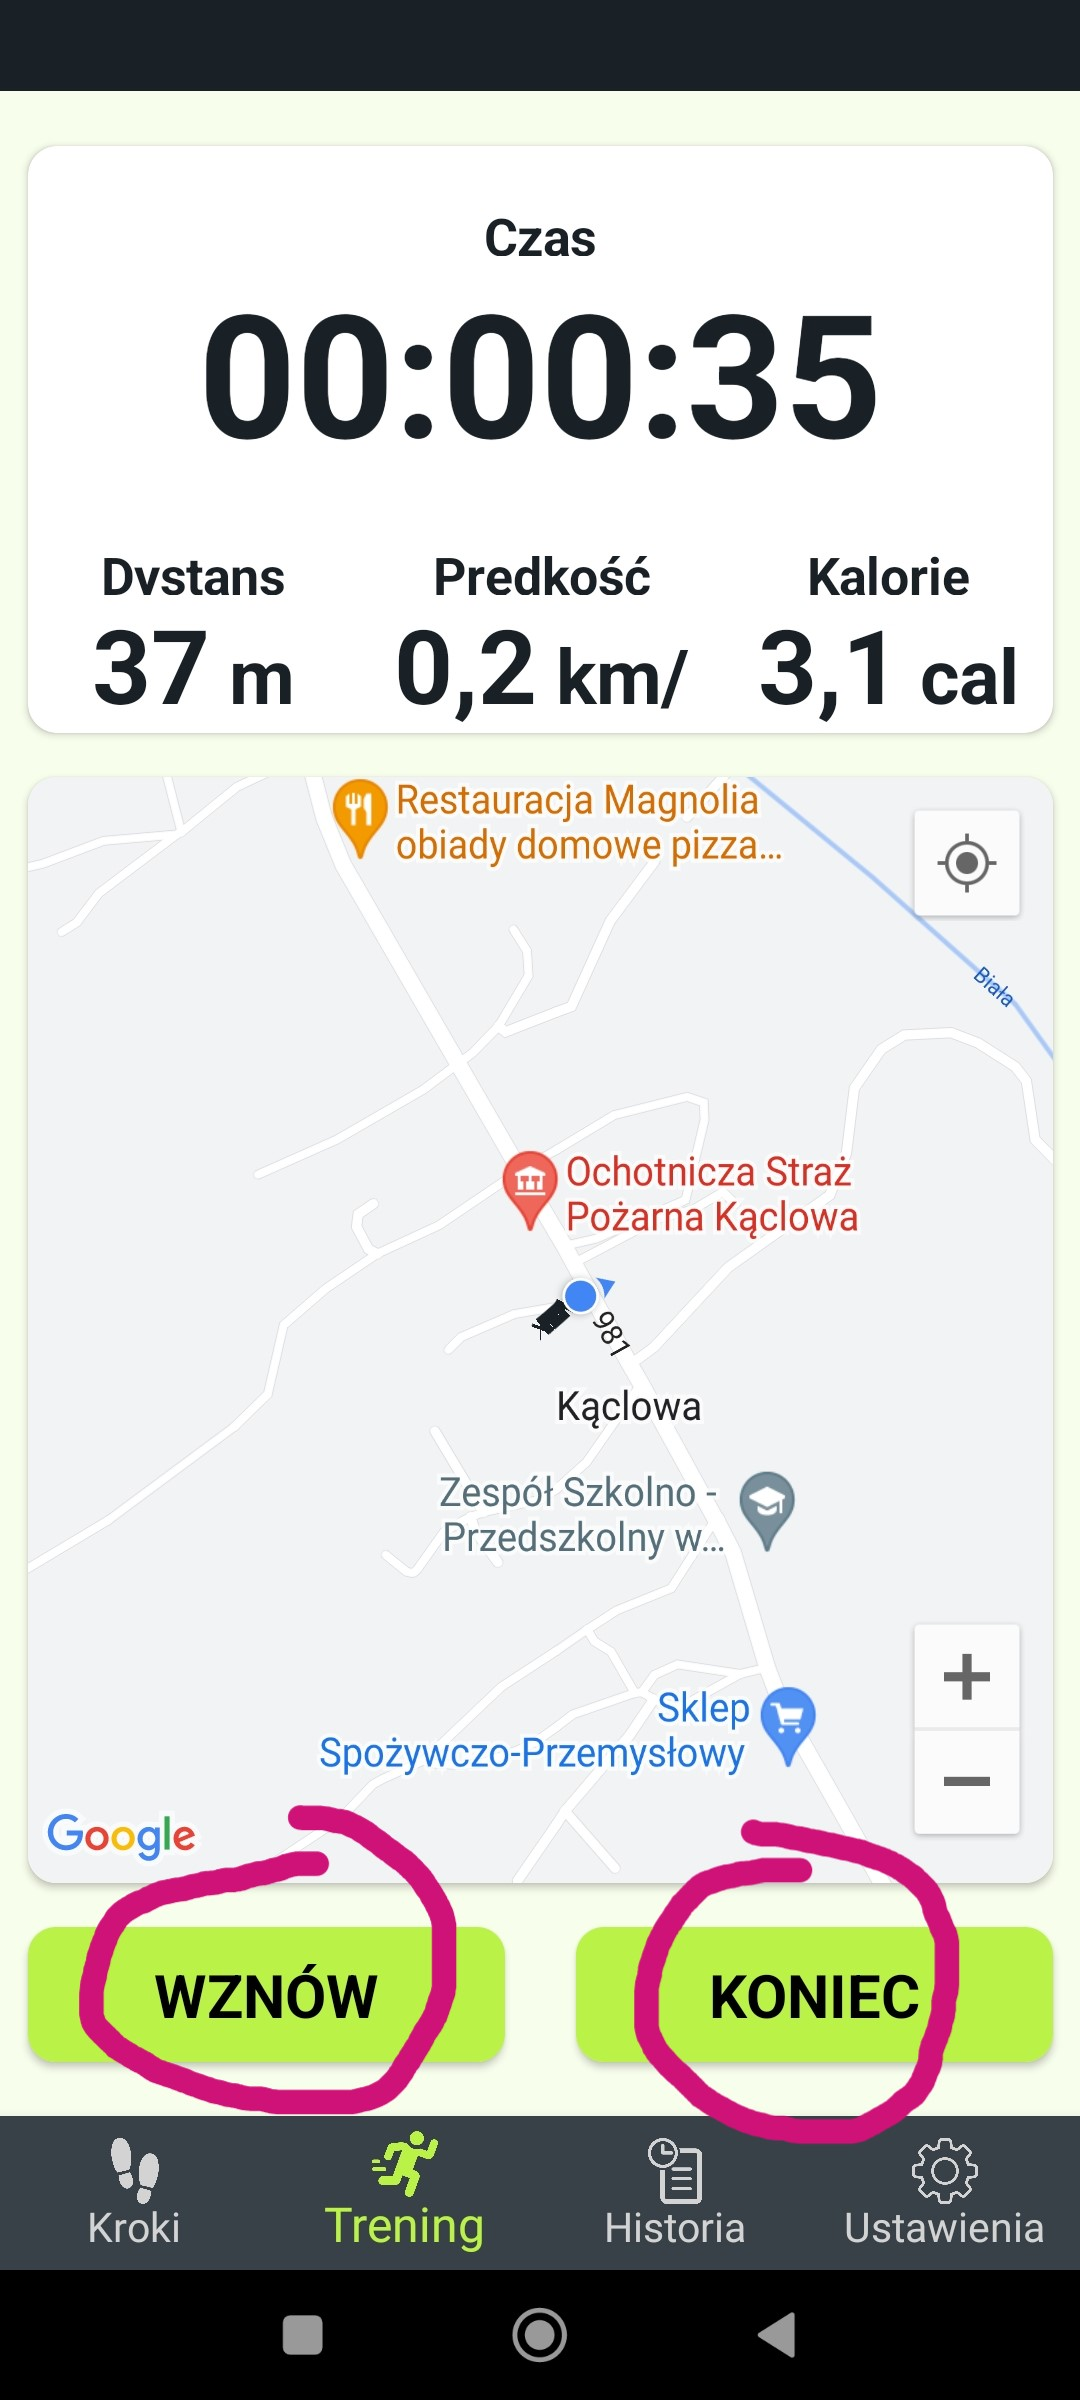
\includegraphics[width=.4\linewidth]{rys/r612.jpg}
		\caption{Wznowienie lub Zakończenie}
		\label{rys:rysunek-r612}
	\end{minipage}%
	\begin{minipage}{.5\textwidth}
		\centering
		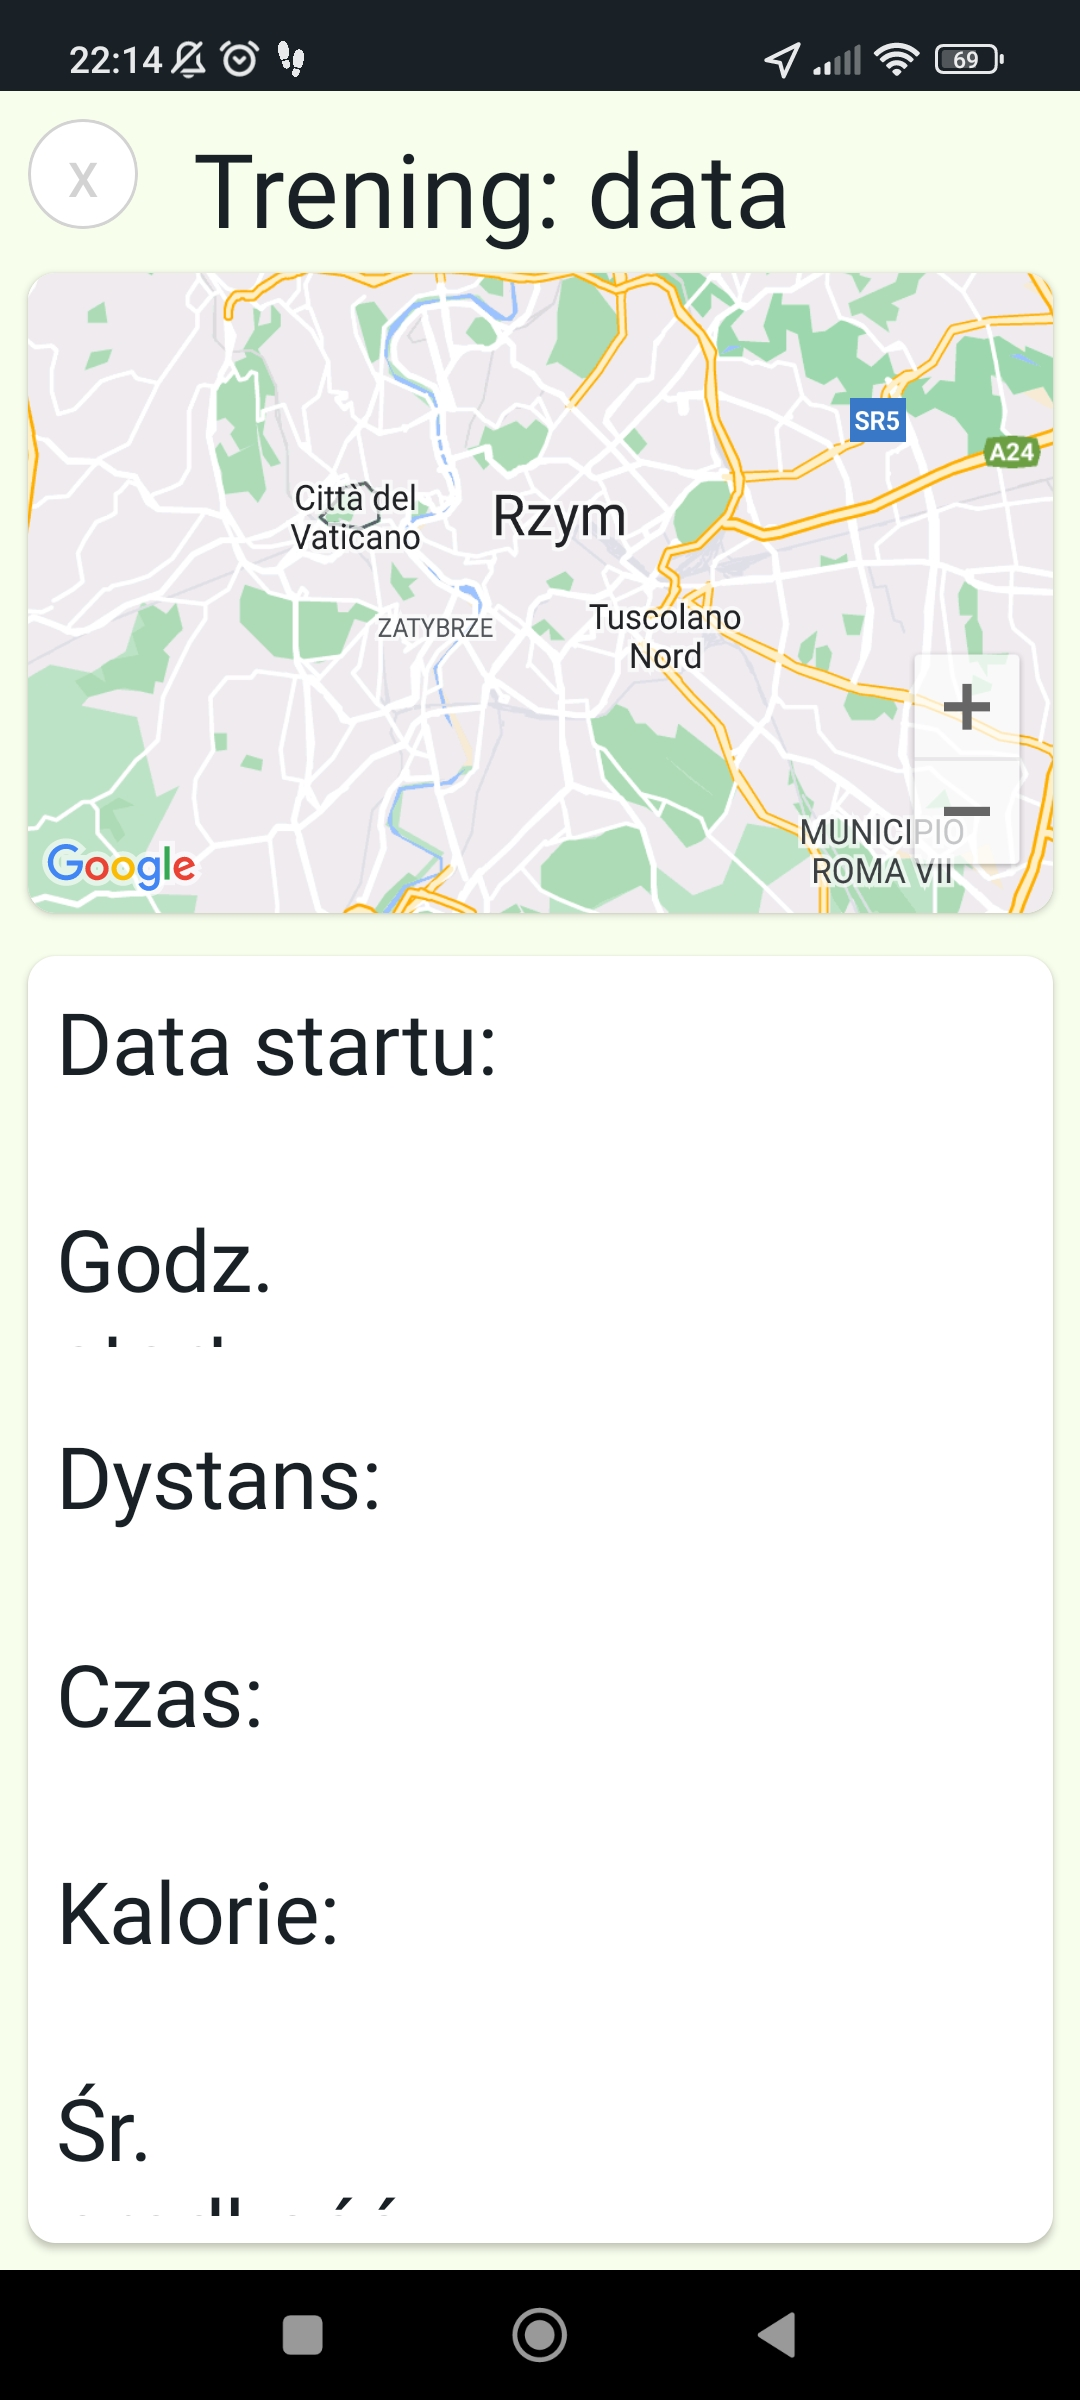
\includegraphics[width=.4\linewidth]{rys/r613.jpg}
		\caption{Ekran podsumowania}
		\label{rys:rysunek-r613}
	\end{minipage}
\end{figure}

Dane te zostają zapisane do historii treningów, którą w każdej chwili możesz obejrzeć poprzez zakładkę Historia (rys. \ref{rys:rysunek-r614}). 
Aby wyczyścić historię treningów, w~zakładce Ustawienia robimy to za pomocą przycisku Wyczyść treningi (rys. \ref{rys:rysunek-r65}). 
Aplikacja ma również opcję ustawiania powiadomień o treningach, abyś nie wypadł z formy:) Wystarczy kliknąc na przycisk Ustaw powiadomienie (rys. \ref{rys:rysunek-r65}) i wpisać godzinę, o której każdego dnia aplikacja ma ci przypominać o treningach (rys. \ref{rys:rysunek-r615}).

\begin{figure}[!htb]
	\centering
	\begin{minipage}{.5\textwidth}
		\centering
		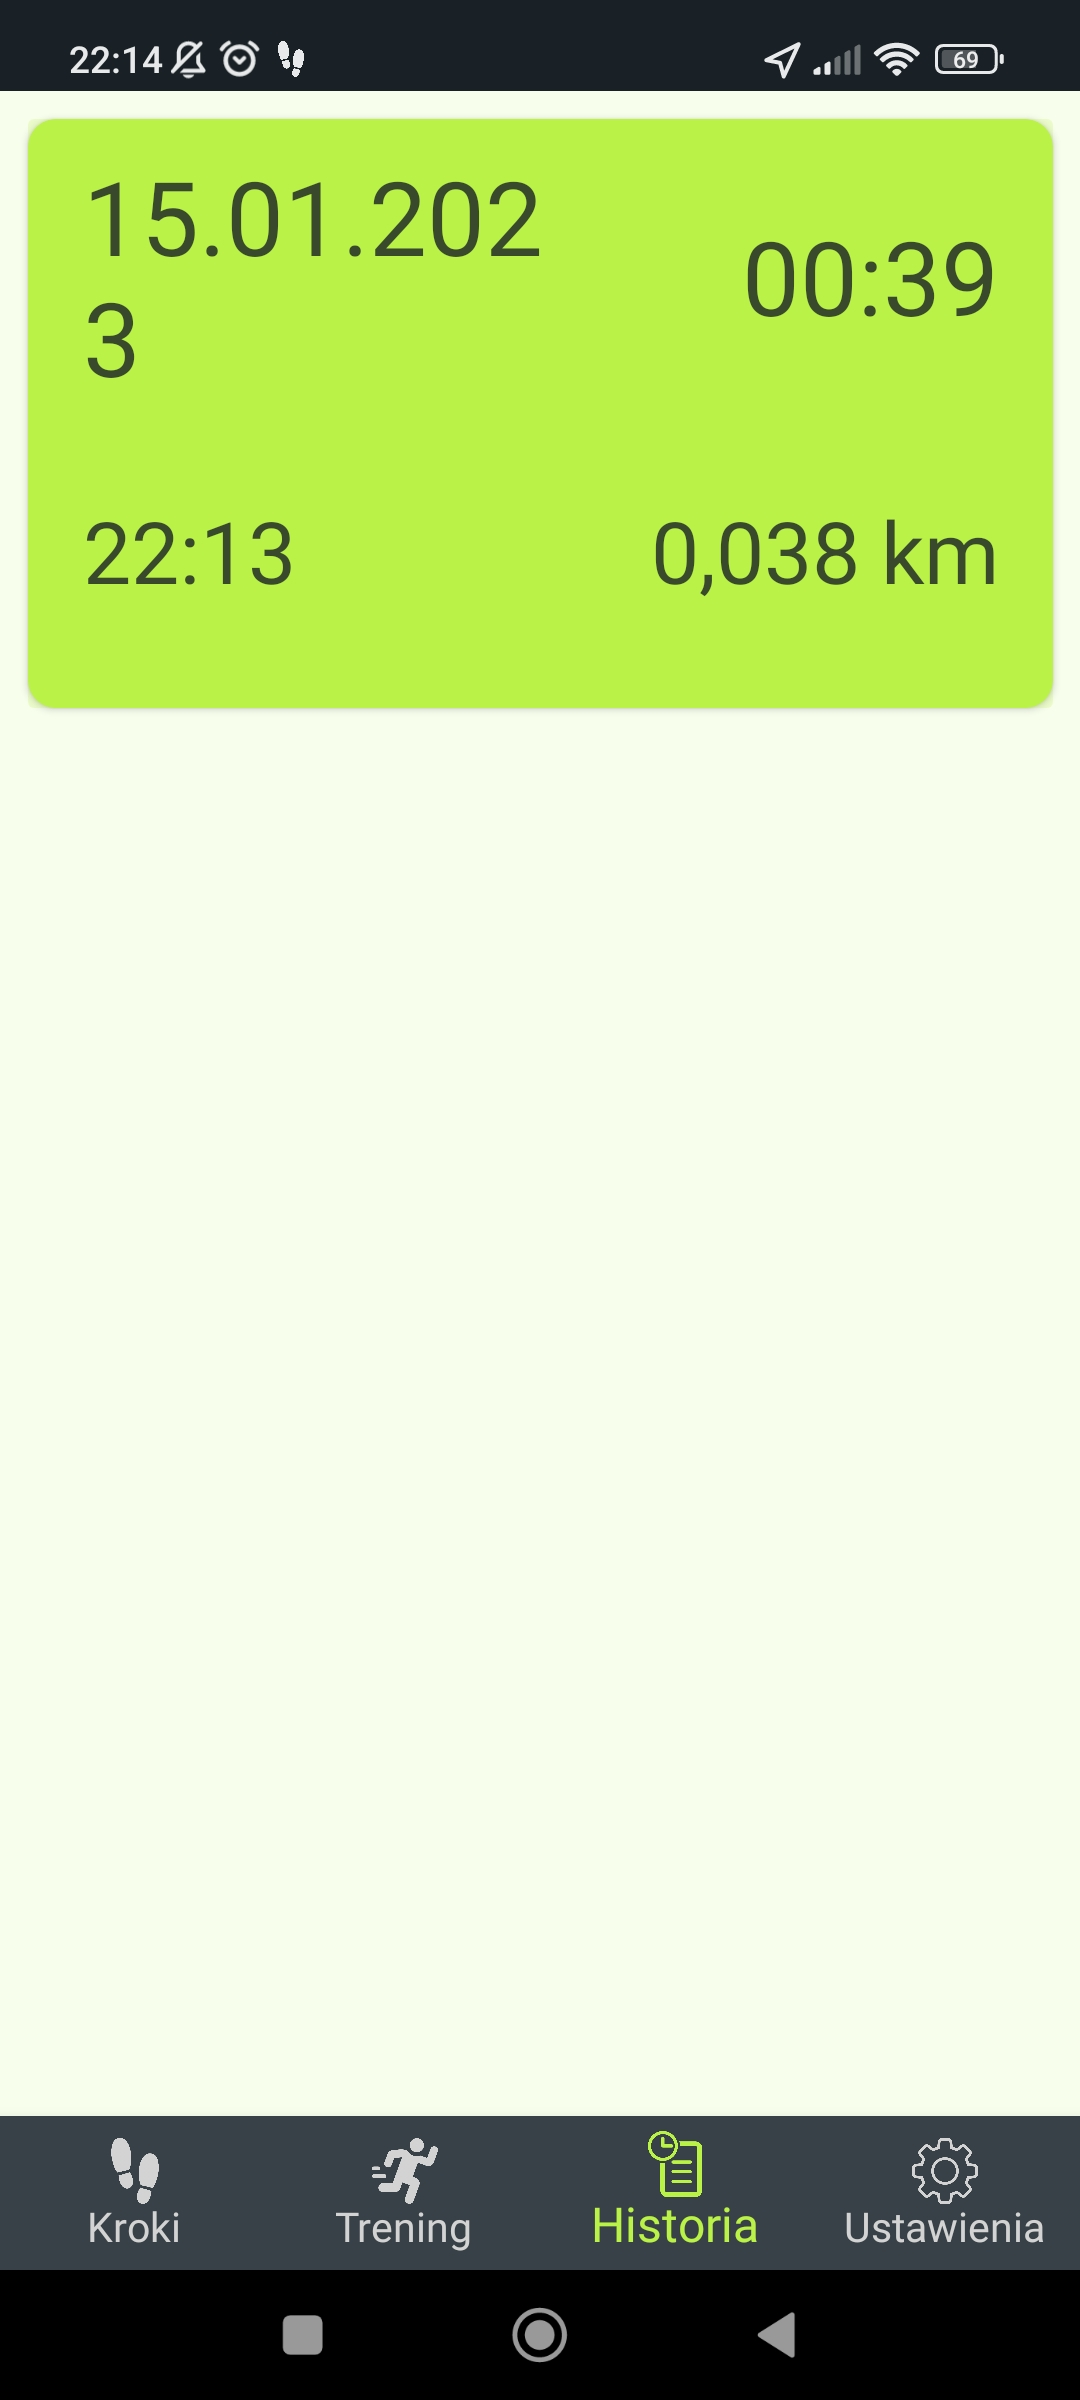
\includegraphics[width=.4\linewidth]{rys/r614.jpg}
		\caption{Zapisanie do historii}
		\label{rys:rysunek-r614}
	\end{minipage}%
	\begin{minipage}{.5\textwidth}
		\centering
		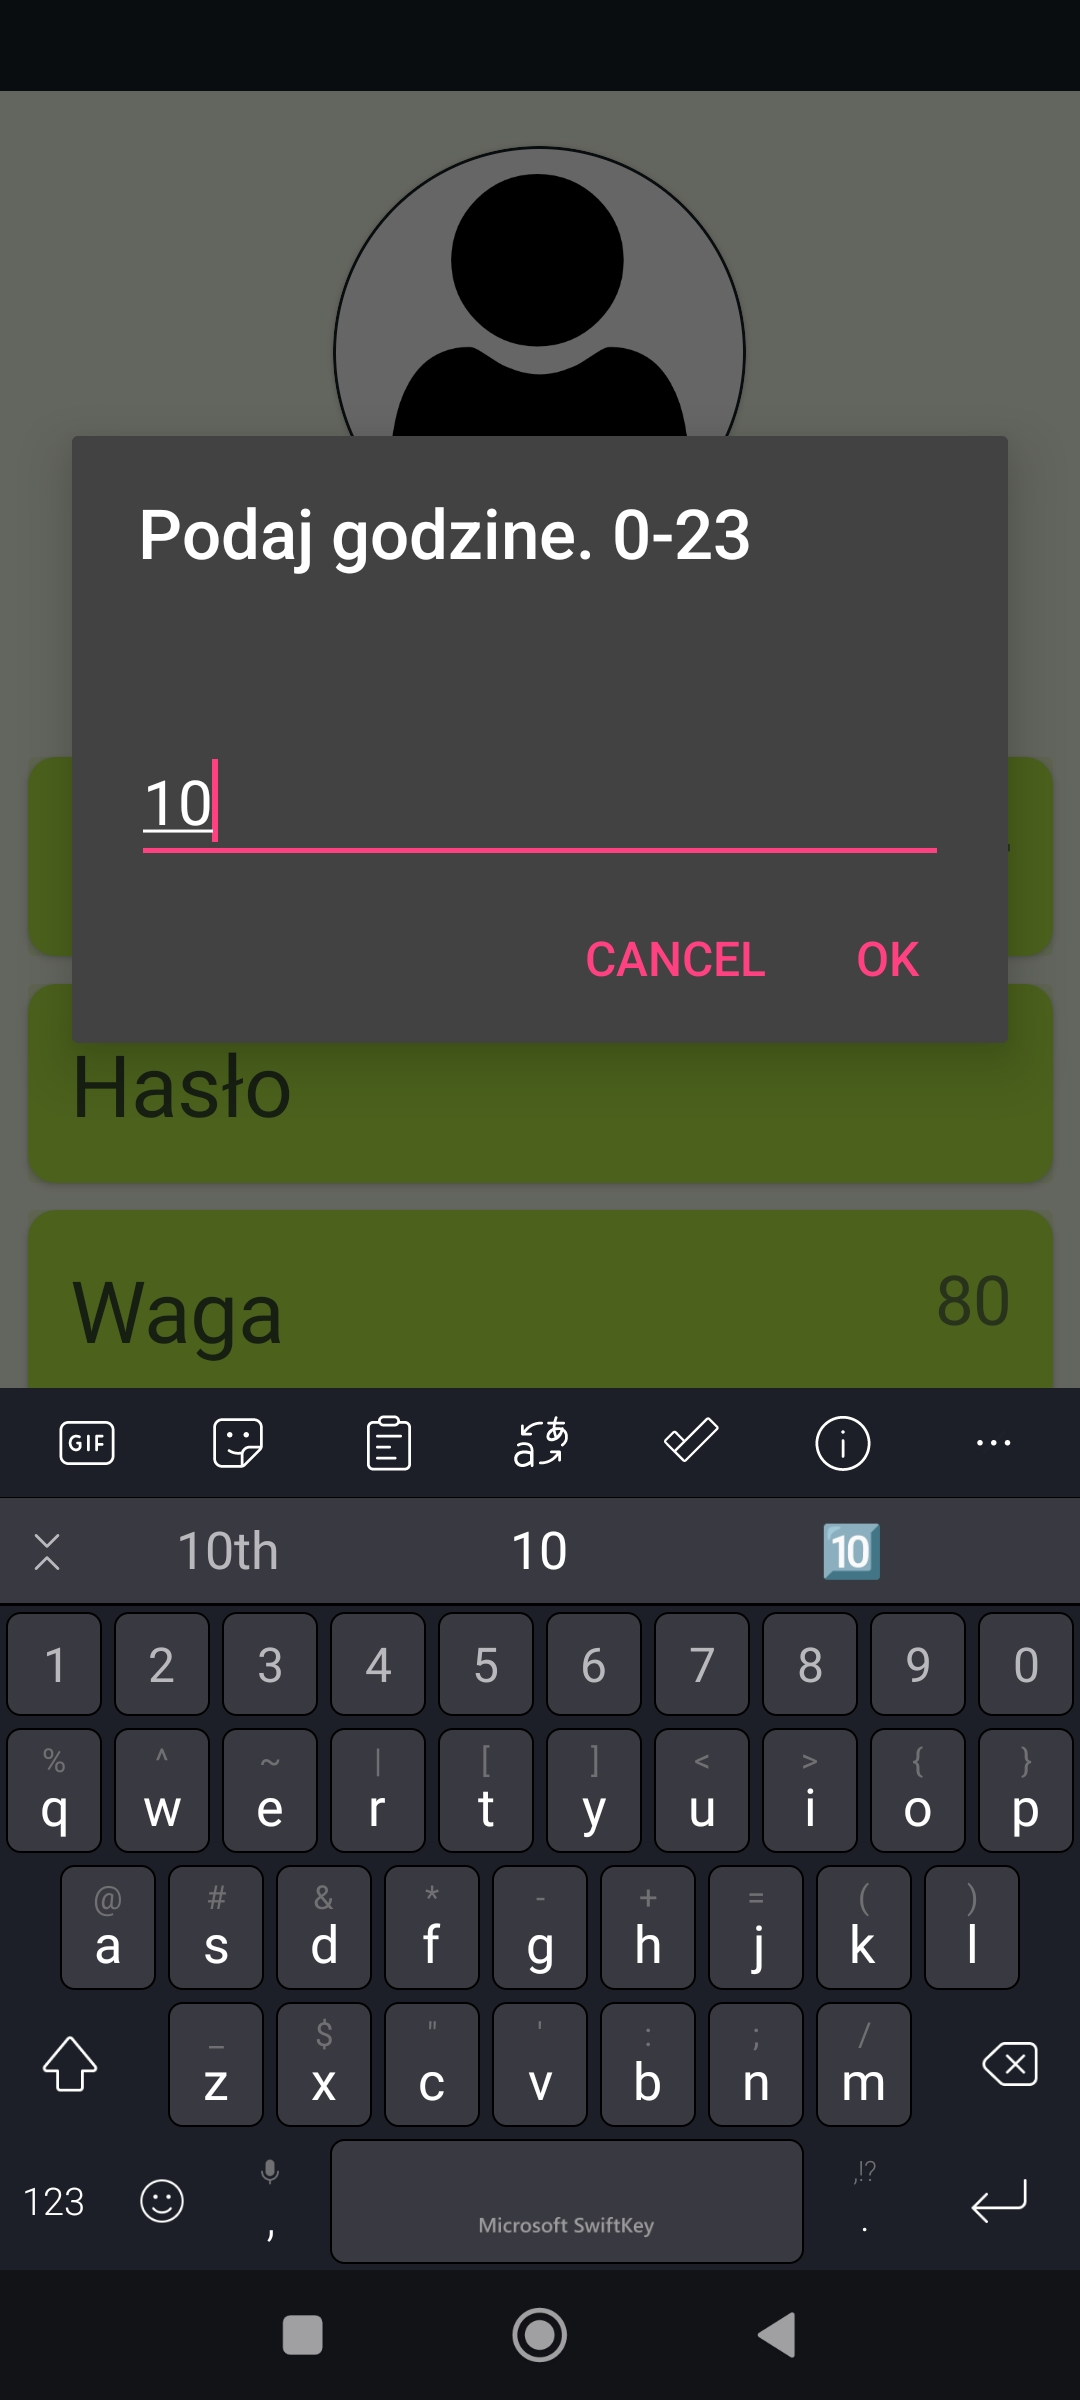
\includegraphics[width=.4\linewidth]{rys/r615.jpg}
		\caption{Ustawienie powiadomienia}
		\label{rys:rysunek-r615}
	\end{minipage}
\end{figure}

Mamy nadzieję, że korzystanie z tej aplikacji sprawi Ci przyjemność, i że pomoże Ci ona osiągnąć Twoje cele fitness!


